\documentclass[sigconf]{acmart}

\usepackage{graphicx} \usepackage{balance} \usepackage{hyperref} \usepackage[all]{nowidow} \usepackage{float}
\usepackage{tikz} \usepackage{tikz-3dplot} \usepackage{nicefrac} \usepackage{algorithm} \usepackage{subcaption}
\usepackage[noend]{algpseudocode} \usepackage{array} \usepackage{pgfplots} \usepackage{booktabs} \usepackage{siunitx}
\usepackage{enumitem} \usepackage[utf8]{inputenc} \usepackage{amsmath} \usepackage{amssymb} \usepackage{filecontents}
\usepackage{amsfonts}

\newcommand{\vv}[1]{#1} % Not doing anything special for vectors right now...
\newcommand{\seq}{\!=\!}
\newcommand{\iFrame}{\mathcal{I}}
\newcommand{\kFrame}{\mathcal{K}}
\everypar{\looseness=-1}

\copyrightyear{2019}
\acmYear{2019}
\setcopyright{acmlicensed}
\acmConference[Santa Cruz '19]{Santa Cruz '19: 31st International Conference on Scientific and Statistical Database Management}{July 23--25, 2019}{Santa Cruz, CA}
\acmBooktitle{Santa Cruz '19: 31st International Conference on Scientific and Statistical Database Management, July 23--25, 2019, Santa Cruz, CA}


\begin{document}
	\title{An Experimental Survey of Evaluation Strategies for Constellation Queries}

    \author{Glenn Galvizo}
    \email{glennga@hawaii.edu}
    \affiliation{%
        \institution{University of Hawaii at Manoa}
        \city{Honolulu}
        \state{Hawaii}
    }

    \author{Lipyeow Lim}
    \email{lipyeow@hawaii.edu}
    \affiliation{%
        \institution{University of Hawaii at Manoa}
        \city{Honolulu}
        \state{Hawaii}
    }
    
	%\begin{abstract}
%    The process of identifying stars is integral toward stellar based orientation determination in spacecraft.
%    Star identification involves matching points in an image of the sky with stars in an astronomical catalog.
%    A unified framework for identification was created and used to analyze six variations of methods based on their
%    approach to star set identification, obtaining a single image to catalog star set match, and uniquely mapping
%    each star in a image star set to a catalog star set.
%    Each method was presented an artificial image, and aspects that were interchangeable among each process were
%    normalized.
%    Given an image with false stars, the Pyramid method has the highest average accuracy and is the fastest of the six.
%    Given an image where each star's true position is distributed randomly (Gaussian noise), the Spherical Triangle
%    method's accuracy is the least sensitive.
%\end{abstract}

\begin{abstract}
    Given a set of query points within an image coordinate system, constellation queries find the matching points in a
    database of known points within a standard coordinate system.
    Constellation queries are an integral part of orientation determination systems used in spacecrafts to orient and
    navigate themselves.
    The query points are bright spots in an image captured by a camera on the spacecraft and the database contains known
    celestial objects in a celestial coordinate system.
    This paper studies six existing constellation query processing strategies (Angle, Interior Angle, Spherical Triangle,
    Planar Triangle, Pyramid, Composite Pyramid) using a unified algorithmic framework and presents an extensive
    experimental evaluation of the six strategies.
    Given an image with false points, the Pyramid strategy has the highest average accuracy and is the fastest of the six.
    Given an image where each point's true position is distributed randomly (Gaussian noise), the Spherical
    Triangle strategy's accuracy is the least sensitive to positional change.
\end{abstract}

	
	\begin{CCSXML}
		<ccs2012>
		<concept>
		<concept_id>10002951.10003317</concept_id>
		<concept_desc>Information systems~Information retrieval</concept_desc>
		<concept_significance>500</concept_significance>
		</concept>
		<concept>
		<concept_id>10002951.10003317.10003325</concept_id>
		<concept_desc>Information systems~Information retrieval query processing</concept_desc>
		<concept_significance>500</concept_significance>
		</concept>
		<concept>
		<concept_id>10002951.10003317.10003359.10003362</concept_id>
		<concept_desc>Information systems~Retrieval effectiveness</concept_desc>
		<concept_significance>500</concept_significance>
		</concept>
		<concept>
		<concept_id>10002951.10003317.10003359.10003363</concept_id>
		<concept_desc>Information systems~Retrieval efficiency</concept_desc>
		<concept_significance>500</concept_significance>
		</concept>
		</ccs2012>
	\end{CCSXML}
	
	\ccsdesc[500]{Information systems~Information retrieval}
	\ccsdesc[500]{Information systems~Information retrieval query processing}
	\ccsdesc[500]{Information systems~Retrieval effectiveness}
	\ccsdesc[500]{Information systems~Retrieval efficiency}
	
	\maketitle

    \keywords{
        information retrieval, performance analysis, query processing
    }

	\section{Introduction}\label{sec:introduction}
Ancient mariners could look up the night sky, point out what stars they were looking at, and navigate across the globe
with precision.
\textit{Star identification algorithm} refers to a computational approach to pointing out which stars
are in the sky.
Given an image of the sky, star identification is matching the bright spots in an image, to stars in an astronomical
catalog.
The device that performs these computations is the star tracker, much like the navigators on the ship.
\textit{Lost-in-space} refers to an additional constraint on the problem: the absence of knowing where we took
the picture and how we pointed the camera.

This problem is most prevalent in designing LEO (low Earth orbit) spacecraft.
In order for a craft to point a payload, direct thrusters, or orient it's solar panels, an accurate
\textit{attitude} (another term for orientation) must be known.
There are a few known landmarks in space where some attitude can be extracted (the Earth, the Sun), but this
requires constant direction towards just these objects.
Star trackers do not limit themselves to a single object, rather they use the entire sky of stars to determine it's
orientation.

There exist roughly 4500 stars in the sky visible to the human eye.
It is computationally expensive to iterate through each combination of stars in the sky, so star identification methods
are used instead.
This paper analyzes six existing methods, all of which involve the following process:
\begin{enumerate}
    \item Given an image of stars.
    \item Identify a select few stars in the image.
    \item Guess how we are oriented.
    \item Identify the rest of the stars in the image.
    \item Finalize and determine our orientation.
\end{enumerate}

Each method's feature uniqueness, permutation order, candidate reduction, and identification process will be
characterized under the introduction of various noise.
The process of identifying blobs in an image, constructing the image coordinate system, and efficiently querying
static databases is not addressed here.

There has been an increasing number of approaches toward stellar attitude determination, but little comparison between
each of these methods in a more controlled manner.
Interchangeable factors are abstracted away (camera hardware, blob detection, etc\ldots) to focus more on how each
method matches stars in an image to a catalog.
	\section{Related Work}\label{sec:relatedWork}
This section serves to give a brief overview into the different approaches to the lost-in-space star identification
problem.
Many of the methods listed here have also been described and compared by
Spratling~\cite{spratling:surveyStarIdentification} and Br\"{a}tt~\cite{bratt:analysisStarIdentification}.

\subsection{Subgraph Isomorphism Approach}\label{subsec:subgraphIsomorphismApproach}
\textit{Subgraph isomorphism} is a NP complete problem which aims to find some 1-to-1 mapping between the vertices
(stars) in two graphs (i.e.\ the catalog and the image) if it exists~\cite{scott:graphIsomorphismProblem}.
Methods that approach the star identification problem as such are the ones analyzed in this paper.

In 1978, Gottlieb developed the Polygon Angular Matching method which identifies 3 stars using interstar
angles~\cite{gottlieb:spacecraftAttitudeDetermination}.
In 1986, Groth introduced a Pattern Matching algorithm for lists of coordinates, which identifies 3 stars using the
relative ratios between each interstar angle and logarithm of this sum~\cite{groth:patternMatchingMethod}.
In 1991, Anderson proposed the use of storing permutations instead of combinations to avoid an additional
identification step at the expense of storage~\cite{spratling:surveyStarIdentification,anderson:autonomousStarSensing}.
In 1992, Renken developed a method which allowed for variable number of image subsets based on interstar angle matching
of 2 to 6 stars~\cite{bratt:analysisStarIdentification,renken:starConstellationMatching}.

In 1993, Baldini introduced a method which identifies $b$ bright stars in an image using five stars and their interstar
angles~\cite{spratling:surveyStarIdentification,baldini:starConstellationMatching}.
In 1994, Scholl proposed using the intesities themselves as features to remove the additional identification step
~\cite{spratling:surveyStarIdentification,scholl:starFieldIdentification}.
In 1995, Liebe developed the Liebe Star ID method which identifies 3 stars using two interstar angles and the
interior angle with one of the stars as the vertex~\cite{liebe:starTrackersAttitudeDetermination}.
Also in 1995, Ketchum developed the second sequential filtering algorithm, which identifies 2 stars using their
brightness~\cite{spratling:surveyStarIdentification,ketchum:onboardStarIdentification}.

In 2004, Mortari first developed the Pyramid method which introduces a special process for determining image star
subsets, a verification step to identify 4 stars, and a "searchless" database access
method to speed up query time~\cite{motari:pyramidIdentification}.
In 2004 and 2006, Cole \& Crassidus developed the Spherical and Planar Triangle methods
respectively which identifies 3 stars using the area and torque formed by the triangles of interstar angles, and a
process for reducing candidates~\cite{coleAndCrassidis:sphericalTriangleMethod, coleAndCrassidis:planarTriangleMethod}.
In 2005, Rousseau et. al introduced the use of the sine of the interior angle of three stars as a feature as well as
the idea of truncating the possible catalog matches based on a computed
attitude~\cite{bratt:analysisStarIdentification,rousseau:starRecognitionAPS}.

In 2007, Kolomenkin et. al developed the voting algorithm, which would accumulate votes for every combination of
two stars in the image if the interstar angle of some pair in the image matched the angle in the
catalog and maps stars based on the number of votes
received~\cite{bratt:analysisStarIdentification,kolomenkin:geometricVoting}.
In 2011, Tichy et. al developed the two-star voting algorithm, which votes in a similar fashion to the voting algorithm
but applies votes toward a single star based off two interstar angles instead of votes toward two stars
~\cite{bratt:analysisStarIdentification,tichy:preliminaryTestsCommericalImagers}.
In 2014, Toloei developed the Novel Stars ID method, which retains all of the key aspects of the Pyramid method but
uses the features from Planar Triangle method~\cite{toloei:compositeIdentification}.

\newcommand{\srightarrow}{\! \rightarrow \!}
\begin{figure}[ht]
    \centering{
    \usetikzlibrary{shapes.geometric, arrows}

% Style for process block.
\tikzstyle{process} = [rectangle, text width=2cm, minimum width=2cm, minimum height=0.5cm,text centered, draw=black,
fill=orange!30]

% Style for terminal block.
\tikzstyle{terminal} = [rectangle, text width=2cm, minimum width=2cm, minimum height=0.5cm,text centered,
draw=black, fill=red!30]

% Style for decision block.
\tikzstyle{decision} = [diamond, text width=1.5cm, minimum width=2.2cm, minimum height=1.8cm,text centered, draw=black,
fill=green!30, inner sep=-12pt]

% Style for line.
\tikzstyle{line} = [draw, -latex']

\begin{tikzpicture}[node distance=1.2cm]
    \node[scale=1](getImage)[terminal]{Get Camera Image};
    \node[scale=1](pickQueryStars) [process, left of=getImage, xshift = -2.2cm] {Pick $d$ Image Stars};
    \node[scale=1](searchCatalog)[process, below of=pickQueryStars, yshift=-0.4cm] {Search Catalog};
    \node[scale=1](confidentInCatalog)[decision, below of=searchCatalog, yshift=-0.4cm] {$\lvert R \rvert > 0$?};
    \node[scale=1](filterCandidates)[process, below of=confidentInCatalog, yshift=-0.4cm] {Filter Candidates};
    \node[scale=1](confidentAfterFilter)[decision, below of=filterCandidates, yshift=-0.4cm] {Confident?};
    \node[scale=1](findMap)[process, below of=confidentAfterFilter, yshift=-0.4cm]{Identify};
    \node[scale=1](confidentInMap)[decision, below of=findMap, yshift=-0.4cm] {Confident?};
    \node[scale=1](returnMap)[terminal, right of=confidentInMap, xshift = 2.2cm] {Return $b, r, f$};

    \draw[->,>=stealth](getImage) -- node[scale=1.3, yshift=-0.3cm]{$I$}(pickQueryStars);
    \draw[->,>=stealth] (pickQueryStars) -- node[scale=1.3, xshift=0.5cm]{$b$}(searchCatalog);
    \draw[->, >=stealth] (searchCatalog) -- node[scale=1.3, xshift=0.5cm, yshift=-0.15cm]{$R$}(confidentInCatalog);
    \draw[->, >=stealth] (confidentInCatalog) -- node[anchor=east, yshift=0.1cm]{Yes}(filterCandidates);
    \draw[->, >=stealth] (filterCandidates) --
    node[scale=1.3, xshift=0.5cm, yshift=-0.15cm]{$r$}(confidentAfterFilter);
    \draw[->, >=stealth] (confidentAfterFilter) -- node[anchor=east, yshift=0.1cm]{Yes} (findMap);
    \draw[->, >=stealth] (findMap) --
    node[scale=1.3, xshift=1cm, yshift=-0.15cm]{$f: b \rightarrow r$} (confidentInMap);
    \draw[->, >=stealth] (confidentInMap) -- node[xshift=0cm, yshift=0.25cm]{Yes} (returnMap);

    \draw[->, >=stealth] (confidentInCatalog.west) -- ++(-1.4cm, 0cm) node[anchor=south, xshift=0.5cm]{No}
    |- (pickQueryStars.west);
    \draw[->, >=stealth] (confidentAfterFilter.west) -- ++(-1.4cm, 0cm) node[anchor=south, xshift=0.5cm]{No}
    |- (pickQueryStars.west);
    \draw[->, >=stealth] (confidentInMap.west) -- ++(-1.4cm, 0cm) node[anchor=south, xshift=0.5cm]{No}
    |- (pickQueryStars.west);
\end{tikzpicture}
    \caption{
    Flowchart depicting the unified identification framework which all methods here follow.
    Given an image $I$, this process returns a bijection $h$ between some subset of the input $b$ and a subset of the
    catalog $r$.
    In the event all subsets are exhausted, the function $h: b \srightarrow \emptyset$ is returned (not depicted).
    } \label{figure:unifiedIdentificationFlowchart}
    }
\end{figure}

\subsection{Pattern Recognition Approaches}\label{subsec:otherApproaches}
The \textit{pattern recognition} approach differs from the subgraph ismorphism approach in that stars themselves exist
as a part of patterns to be matched across the catalog and the image~\cite{bittanti:starIdentificationStudy}.
This is the other main approach to the identification problem, most of which is composed of grid algorithms
~\cite{lee:modifiedGridAlgorithm,padgett:gridAlgorithm} and neural network
approaches~\cite{lindsey:neuralNetworkMethods,alvelda:neuralNetworkStar}.
%There exist several methods outside of the norm that appear to perform well, the most notable being Quan's Adaptive
%Ant Colony method~\cite{}.
	\newcommand{\algorithmautorefname}{Algorithm}
\newcommand{\algeqref}[1]{\hyperref[#1]{Eq.~\ref*{#1}}}
\algnewcommand{\LineComment}[1]{\State \(\triangleright\) #1}
\algrenewcommand\algorithmicindent{0.35cm}
\newcommand{\bigO}{\mathcal{O}}
\newcommand{\abs}[1]{\left| #1 \right|}
\newcommand{\set}[1]{\left\{ #1 \right\}}
\MakeRobust{\Call}

\newfloat{algorithm}{t}{lop}
\restylefloat{algorithm}

\section{Star Identification Methods}\label{sec:starIdentificationMethods}
Six different approaches to star identification are described in this section.
The majority of the literature specifying these methods do not include pseudocode, rather they specify descriptions 
of specific processes used by each method.
Each algorithm is composed of these processes, structured to follow a general identification flow.
When the description did not specify a step in this flow, a naive or existing approach from another method was used.
Several deviations to the algorithms from the original literature were introduced from newer literature to evaluate
the effectiveness of these changes.

\subsection{Unified Identification Framework}\label{subsec:unifiedIdentification}
Each identification method is presented with an image $I$ of size $n$ containing all the stars in the image reference,
as well as a catalog of known stars $K$.
All stars in $I$ exist in the body frame $\iFrame$, and all stars in $K$ exist in the inertial frame $\kFrame$.
The goal of each method is to find some bijection between a subset of the image stars $b$ and a subset
of the catalog stars $r$.
This function is denoted as $h$ with domain $b$ and codomain $r$.
Complete identification of all stars in each image is not the focus.

\begin{subequations}
    Every algorithm starts with some combination from all possible $d$ combinations of $n$ stars $C(n, d)$, where
    $d$ is the size of the image subset that specific identification method uses.
    $b$ is selected using one of these combinations.
    For an identification method that uses $d\seq2$ stars to determine the mapping in an image of $n\seq 4$ stars,
    the combinations of $I$ are:
    \begin{align}
        C(4, 2) \text{ of } I &= \set{\set{\vv{I_1}, \vv{I_2}}, \set{\vv{I_1}, \vv{I_3}}, \ldots,
        \set{\vv{I_3}, \vv{I_4}}} \\
        C(4, 2) \text{ of } I &= \set{ b_1, b_2, \ldots, b_6 }
    \end{align}
\end{subequations}

\begin{subequations}
    There exists a set $K^d$, composed of $d$ sized sets of all possible combinations (or permutations) of stars
    from the catalog $K$.
    Using certain features of the image star subset, the entire $K^d$ set is filtered to a set of catalog star
    candidates $R$.
    This is known as the catalog query step.
    Referencing the same $d\seq 2$ identification method as before, an image subset $b \seq \set{\vv{I_1},
    \vv{I_2}}$ may yield the candidates in~\autoref{eq:catalogCandidateExample}:
    \begin{align}
        \label{eq:catalogCandidateExample}
        R &= \set{ \set{\vv{K_{104}}, \vv{K_{899}}}, \set{\vv{K_{7622}}, \vv{K_{7771}}}, \ldots) } \\
        R &= \set{ r_1, r_2, \ldots }
    \end{align}
\end{subequations}

Through some filter process or restriction criteria for $R$ itself, a single set $r$ from the catalog star candidates is
eventually selected.
This may require going through multiple catalog candidate sets and repeating the catalog query step.
This is known as the $r$ selection step.
For a process with the $R$ restriction criterion of $|R| \seq 1$, the following sequence
of events may occurring before finding a single $r$ set.
\begin{align*}
    &t = 1, \text{ query with } b^{(1)}, \text{ get } R^{(1)} = \{\vv{r_{11}}, \vv{r_{12}}, \ldots\}. \\
    &t = 2, \ \abs{ R^{(1)} } \neq 1, \text{ criterion not met. } \\
    &t = 3, \text{ choose new image subset } b^{(2)}. \\
    &t = 4, \text{ query with } b^{(2)}, \text{ get } R^{(2)} = \{\vv{r_{21}}\}. \\
    &t = 5, \ \abs{ R^{(2)} } = 1, \text{ criterion met. } \\
    &t = 6, \text{ return } r, r \in R^{(2)} (\text{sole element in } R^{(2)} ).
\end{align*}

From here, a bijection $h : b \srightarrow r$ is determined that maps each star found in the image star subset to a
single star in the catalog candidate set.
If we are not confident in $h$ at this point, another image star subset is chosen and the process is repeated.
If we are confident in $h$, then $b$, $r$, and $h$ are returned.
This process is detailed in~\autoref{figure:unifiedIdentificationFlowchart}.
In the event no map is determined, an error is raised and the function $h : b \srightarrow \emptyset$ is returned
instead.

% Leaving this out for now. The flowchart should explain the process better.
%\begin{algorithm}[ht] \setstretch{1.0}[H]
%    \caption{Generic Star Identification Method} \label{algorithm:genericStarIdentification}
%    \begin{algorithmic}[1]
%        \Procedure{Identify}{}
%        \State $I \gets $ all stars from image
%        \For{$c \in r_k^{|I|}$}
%        \State $b \gets \{I(c_1), I(c_2), I(c_3), \dots, I(r_k)\}$
%        \State $R \gets $ catalog star sets, each set of size $=k$
%        \State $r \gets $ a single set from $R$ that matches $b$
%        \State $a \gets $ a map between $b$ and $r$
%        \\
%        \If{the steps above are successful}
%        \State \textbf{return} $a$
%        \EndIf
%        \EndFor
%        \EndProcedure
%    \end{algorithmic}
%\end{algorithm}

% Citation: https://digitalcommons.usu.edu/cgi/viewcontent.cgi?article=2723&context=etd AND Gottlieb.
\subsection{Angle Method}\label{subsec:angleMethod}
\newcommand{\invalidBijection}{\If{$\forall \ \vv{b^\star}, \ \vv{b^\star} \in b \land h\left(\vv{b^\star}\right)
\neq \emptyset$}}
\begin{algorithm}
    \caption{Angle Identification Method} \label{algorithm:angleIdentification}
    \begin{algorithmic}[1]
        \Function{FPO}{$P$, $I$, $A$}
        \State $I' \gets$ stars in $I$ rotated by $A$
        \State $\bar{P} \gets $ \{$p \in P \ | \ \exists \ i \ (i \in I' \land \theta (i, p) < 3\sigma_o)$\}
        \State \textbf{return} $\bar{P}$ \Comment Stars in $P$ that \textit{overlay} with $I'$.
        \EndFunction
        \\
        \Function{DMT}{$b, r, I$}
        \State $H \gets $ all possible bijections of $b$ and $r$
        \State $P \gets $ all stars in catalog near $r$, $M \gets \emptyset$
        \For {$h \in H$}
        \State $A \gets $ \Call{TRIAD}{$h, b, r$}, $M_h \gets $ \Call{FPO}{$P, I, A$}
        \EndFor
        \If{$|M_0| = |M_1| = \ldots = \abs{M_\abs{M}}$}
        \State \textbf{return} $h : b \rightarrow \emptyset $ \Comment Not confident in result.
        \Else
        \State \textbf{return} $h \in H$ associated with largest set in $M$
        \EndIf
        \EndFunction
        \\
        \Function{Identify}{$I, K^2$}
        \For{$i \gets 1 \text{\textbf{ to }} n$} \Comment Iterate through $C(n, 2)$.
        \For{$j \gets i + 1 \text{\textbf{ to }} n - 1$}
        \State $b \gets \left(\vv{b_i}, \vv{b_j}\right)$, $R \gets \{ r \mid r \in K^2 \land P_\theta(r, b) \}$
%        \State $R \gets $ catalog pairs that meet~\algeqref{eq:angleRequirement} with $b$
        \If{$\lvert R \rvert = 1$}
        \State $h \gets $ \Call{DMT}{$b, R_1, I$} % TODO: Maybe change this notation...
        \invalidBijection
        \State \textbf{return} $b, r, h$
        \EndIf
        \EndIf
        \EndFor
        \EndFor
        \EndFunction
    \end{algorithmic}
\end{algorithm}

Given a set of stars from the image $I$, $d \seq 2$ stars are selected to obtain the $b$
set~\cite{gottlieb:spacecraftAttitudeDetermination}.
The original literature does not specify how to choose the image subset, so the naive approach is taken.
The selection order is governed by lines (2) and (3) in~\autoref{algorithm:angleIdentification}.
This fixes the star $\vv{b_1}$ in $b$ for $n$ image star subset selections, while constantly changing
$\vv{b_2}$ for every new $b$ choice.
An example sequence of pairs is depicted below for $n \seq 3$ stars.
\begin{equation}
    C(3, 2) \text{ of } I = \left(\set{\vv{I_1}, \vv{I_2}}, \set{\vv{I_1},\vv{I_3}}, \set{\vv{I_2},\vv{I_1}},
    \ldots \right)
\end{equation}

The catalog query step searches the $K^2$ catalog for pairs such that the angular separations of the catalog pairs
are close to the angular separation of the image star subset~\cite{bratt:analysisStarIdentification}.
For the image star subset, the origin of the angular separation calculation $\theta(b)$ is the focal point of the lens
itself.
For a catalog star candidate set, the origin of this calculation $\theta(r)$ is the center of the Earth.
To obtain $R$, the predicate $P_\theta(r, b)$ is used to filter the $K^2$ catalog:
\begin{equation}\label{eq:angleRequirement}
    P_{\theta}(r, b) : \left\lvert \theta(r) - \theta(b)\right\rvert < 3 \sigma_\theta
\end{equation}
where $\sigma_{\theta}$ represents the deviation of the uncertainty between the $\theta$ computation with star
sensor measurements and the same $\theta$ computation with stars defined in the catalog.
Assuming the noise follows a Gaussian distribution, it follows that 99.7\% of all true pairs will be within this range
~\cite{coleAndCrassidis:sphericalTriangleMethod}.

Once the catalog candidates are obtained, the $\abs{R} \seq 1$ criterion is imposed, repeating this process until only
one candidate exists in $R$.
This sole element $\vv{R_1}$ is then selected to be $r$.

\begin{subequations}
    To determine the most likely bijection $h$, we follow Needlemen's implementation of the method and perform a
    \textit{direct match test} (DMT)~\cite{tappe:starTrackerDevelopment,needelman:stellarAttitudeAcquisition}.
    Given an image star pair $b$ and a catalog star pair $r$ for, the following is proposed:
    \begin{equation}
    h_1 : h_1\left(\vv{b_1}\right) \rightarrow \vv{r_1}, h_1\left(\vv{b_2}\right) \rightarrow \vv{r_2}
    \end{equation}
    Wahba's problem is then solved using the TRIAD method to obtain a rotation $A_1$ between the image and catalog
    frames.
    This process is repeated for the other possible permutation to obtain a second rotation $A_2$:
    \begin{equation}
        h_2 : h_2\left(\vv{b_1}\right) \rightarrow \vv{r_2}, h_2\left(\vv{b_2}\right) \rightarrow \vv{r_1}
    \end{equation}
\end{subequations}
The most likely attitude is determined by the \Call{FPO}{} method, which returns how many stars from $I$ align with
$K$ given rotation $A_1$ or $A_2$.
The bijection with the most stars is then returned.
If all bijections return sets with the same size, then we are not confident in any of our choices and
return the function $h: \vv{b} \rightarrow \emptyset $.

%The \Call{FPO}{} method determines the number of stars from $I$ in the body frame $\iFrame$ align with $C$ in the
%inertial frame $\kFrame$.
%More stars are selected from the catalog that are near the original subset $r$, denoted as $P$.
%The \Call{FPO}{} method then filters out stars in set $P$ that do not overlay with some star in $I'$, the image set
%rotated by some rotation $q$.
%An additional term $\sigma_o$ is defined, which defines how selective this filter.
%$\sigma_o$ can also be thought of as an assumption of the noise associated with the rotation $q$.

Accessing the catalog is the most expensive operation for all of the identification methods.
Consequently, the running time of this algorithm $T_{angle}$ can be described in terms of the number of queries and
the number of entries that exist in the $K^2$ catalog.
There exist $2n^2$ catalog accesses at worst, requiring two catalog accesses (query step and \Call{DMT}{} calls) for
each combination of pairs in $I$.
The $\log (m_2)$ term describes the number of comparisons until $r$ sets are found and are able to be returned.
Given a B+ tree indexed database with $\abs{K^2} \seq m_2$ elements, no more than $\bigO \left( \log(m_2) \right)$
comparisons are required~\cite{patel:advanceTreeStructures}.
%\begin{equation}\label{eq:complexityAnglePart1}
%    T_{angle} = \bigO\left(C(n, 2) \cdot n \cdot \log(m_{angle}) \right)
%\end{equation}
%We expand the combination term to get:
%\begin{equation}
%    C(n, 2) = \frac{n(n - 1)}{2} = \frac{n^2}{4} - \frac{n}{4}
%\end{equation}
%~\autoref{eq:complexityAnglePart1} then simplifies to~\autoref{eq:complexityAngle}:
\begin{equation}\label{eq:complexityAngle}
    T_{angle} = \bigO\left( n^2 \cdot \log(m_2) \right)
\end{equation}

All methods associated with the Angle method are written in~\autoref{algorithm:angleIdentification}.

\subsection{Dot Angle Method}\label{subsec:dotAngleMethod}
\begin{algorithm}
    \caption{Dot Angle Identification Method} \label{algorithm:dotAngleIdentification}
    \begin{algorithmic}[1]
        \Function{Identify}{$I, \bar{K^3}$}
        \For{$c \gets 1 \text{\textbf{ to }} n$}  \Comment Iterate through all of $I$.
        \State $\theta_I \gets \{\theta(\vv{b_c}, \vv{b_i}) \mid \vv{b_i} \in I\}$ \Comment $\theta$
        (all stars, $\vv{b_c}$).
        \State $\vv{b_{c1}} \gets \vv{b_i}$ associated with smallest $\theta$ in $\theta_I$
        \State $\vv{b_{c2}} \gets \vv{b_i}$ associated with 2nd smallest $\theta$ in $\theta_I$
        \State $b \gets \left(\vv{b_c}, \vv{b_{c1}}, \vv{b_{c2}}\right)$, $R \gets \set{ r \mid r \in \bar{K^3} \land
        P_{\theta, \phi}(r, b) }$
        \If{$\lvert R \rvert = 1$}
        \State \textbf{return} $b, r, h: h\left(\vv{b_c}\right) \rightarrow \vv{r_c}, h\left(\vv{b_{c1}}\right)
        \rightarrow \vv{r_{c1}},$
        \State \ \ \ \ \ \ \ \ \ \ \ \ \ \  \ \ \ \ \ \ $h\left(\vv{b_{c2}}\right) \rightarrow \vv{r_{c2}}$
        \EndIf
        \EndFor
        \EndFunction
    \end{algorithmic}
\end{algorithm}

Given a set of stars from the image $I$, a central star $\vv{b_c}$ is selected.
A new central star selection does not involve generating permutations like the Angle method, rather it involves
iterating through $I$ in a sequential manner.
The two closest stars in the image to the central star are selected next, denoted as $\vv{b_{c1}}$ and $\vv{b_{c2}}$
~\cite{liebe:starTrackersAttitudeDetermination}.

The catalog query step searches the $\bar{K^3}$ catalog for trios such that the features of the catalog trios are
close to the same features of the image subset~\cite{bratt:analysisStarIdentification}.
Unlike the Angle method's $K^d$ set, $\bar{K^d}$ is defined to be all \textit{permutations} of size $d$ rather than
combinations.
These features are defined as the angular separation between the first closest star and the central star
($\theta\left(\vv{b_{c1}}, \vv{b_c}\right)$ vs. $ \theta\left(\vv{r_{c1}}, \vv{r_c}\right)$), the
angular separation between the second closest star and the central star, ($\theta\left(\vv{b_{c2}},
\vv{b_c}\right) $ vs. $\theta\left(\vv{r_{c2}}, \vv{r_c}\right)$),
and the angular separation between the two closest stars with the central star as the origin instead of the Earth or 
focal point ($\phi(b) $ vs. $ \phi(r)$).
To obtain $R$, the predicate $P_{\theta, \phi}(r, b)$ is used to filter the $\bar{K^3}$ catalog:
\begin{equation}
    \begin{aligned}
        P_{\theta, \phi} (r, b): \left\lvert \theta(\vv{r_{c1}}, \vv{r_c}) - \theta(\vv{b_{c1}}, \vv{b_c})\right\rvert
        &< 3 \sigma_{\theta} \ \land \\ \left\lvert \theta(\vv{r_{c2}}, \vv{r_c}) - \theta(\vv{b_{c2}}, 
        \vv{b_c})\right\rvert &< 3 \sigma_{\theta} \ \land \\ \left\lvert \phi(r) - \phi(b)\right\rvert &< 3 
        \sigma_\phi \ \land \\\theta(\vv{r_{c1}}, \vv{r_c}) &< \theta(\vv{r_{c2}}, \vv{r_c})
    \end{aligned}
\end{equation}
where $\sigma_{\theta}$ and $\sigma_{\phi}$ represent the deviation of the uncertainty between the $\theta$ and $\phi$
computations with the star sensor measurements and the same $\theta$ and $\phi$ computations with stars defined in the
catalog.

The original literature states that this should be repeated for all $b$ sets.
Given that complete identification of $I$ is not the goal, this method has been adjusted to query with one $b$ at a
time.
After finding some $R$ that meets the same $R$ criterion as the Angle method, the bijection:
\begin{equation}
    h: h\left(\vv{b_1}\right) \rightarrow \vv{r_1}, h\left(\vv{b_2}\right) \rightarrow \vv{r_2}, h\left(\vv{b_3}\right)
    \rightarrow \vv{r_3}
\end{equation}
is constructed and returned.
Tololei's implementation imposes the last term in predicate $P_{\theta, \phi}(r, b)$ at query time (last term in)
and borrows from Anderson by searches all permutations instead of combinations, removing the need for a star
mapping procedure (e.g.\ direct match test)~\cite{toloei:compositeIdentification, anderson:autonomousStarSensing}.
Storing permutations does increase the storage required for the $\bar{K^3}$ catalog though, which begs the question,
``Does this extra space aid in accuracy or runtime?''.

%The star trios in the catalog star candidates represent potential catalog maps for the image star trio $(b_i, b_j,
%b_c)$.
%Liebe's original method states that this process should be repeated for all stars in the image, meaning that all
%stars will be the central star at one point
%By the end, each star in the image will have accrued a set of possible catalog matches $Y$.
%The complete $I \rightarrow R$ map is found by picking the most frequent catalog star appearing in each $Y$
%set~\cite{liebe:starTrackersAttitudeDetermination,bratt:analysisStarIdentification}.
%
%To more closely follow the generic star identification flow, we modified the Dot Angle method to not store $Y$,
%requiring that only one central star choice is needed to acquire a total match.
%If a confident match is not found by the first central star, then the search process will be repeated until such a
%match is found.

The running time of this algorithm $T_{dot}$ is depicted below, again described in terms of the number of queries
and $\bar{K^3}$ catalog entries:
\begin{equation}\label{eq:dotComplexity}
    T_{dot} = O\left( n \cdot \log(\bar{m_3}) \right)
\end{equation}
where $\bar{m_3}$ is the size of the $\bar{K^3}$ catalog.

This entire method is described in~\autoref{algorithm:dotAngleIdentification}.

\subsection{Spherical Triangle Method}\label{subsec:sphericalTriangleMethod}
\begin{algorithm}
    \caption{Triangle Method Identification} \label{algorithm:triangleIdentification}
    \begin{algorithmic}[1]
        \Function{PartialMatch}{$R, \bar{R}$}
        \ForAll {$\bar{r} \in \bar{R}$}
        \LineComment $\bar{r}$ and $r$ share two stars.
        \If {$\exists \ r \ | \ (r \in R \land |r \cap \bar{r}| = 2)$}
        \State $R_{new} \gets \bar{R} \cup \{\bar{r}\}$
        \EndIf
        \EndFor
        \State \textbf{return} $R_{new}$
        \EndFunction
        \\
        \Function{Pivot}{$\vv{b_i}, \vv{b_j}, \vv{b_k}, R$}
        \State $b \gets (\vv{b_j}, \vv{b_j}, \vv{b_k})$, $\bar{R} \gets \set{ \bar{r} \mid \bar{r} \in K^3
        \land P_{a, \tau}(\bar{r}, b) }$
        \State $R' \gets $ \Call{PartialMatch}{$R, \bar{R}$}
        \If{$\abs{R'} = 1 \lor \abs{R'} = 0 $}
        \State \textbf{return} $R'$ \Comment $R'$ is either $\emptyset$ or a single $r$.
        \Else
        \State $\vv{\beta} \gets \text{an unused star in this pivot}$
        \State \textbf{return} \Call{Pivot}{$\vv{b_i}, \vv{b_j}, \vv{\beta}, R'$}
        \EndIf
        \EndFunction
        \\
        \Function{Identify}{$I, K^3$}
        \For{$i \gets 1 \text{\textbf{ to }} n$}  \Comment Iterate through $C(n, 3)$.
        \For{$j \gets i + 1 \text{\textbf{ to }} n - 1$}
        \For{$k \gets j + 1\text{\textbf{ to }} n - 2$}
        \State $b \gets \left(\vv{b_i}, \vv{b_j}, \vv{b_k}\right)$
        \State $R \gets \set{ r \mid r \in K^3
        \land P{a, \tau}(r, b) }$
        \If{$|R| \neq 1$} \Comment Pivot if necessary.
        \State $R \gets $ \Call{Pivot}{$\vv{b_i}, \vv{b_j}, \vv{b_k}, R$}
        \EndIf
        \If{$R \neq \emptyset$} \Comment Verify the pivot's success.
        \State $h \gets $ \Call{DMT}{$b, R_1, I$}
        \invalidBijection
        \State \textbf{return} $b, R_1, h$
        \EndIf
        \EndIf
        \EndFor
        \EndFor
        \EndFor
        \EndFunction
    \end{algorithmic}
\end{algorithm}

Given a set of stars from the image $I$, $d \seq 3$ stars are selected to obtain the $b$ set.
Again, the $b$ selection is not specified here so we assume the naive approach with $C(n, 3)$ combinations.
The star $\vv{b_1}$ is fixed in $b$ for $n^2$ image star subset selections, the star $\vv{b_2}$ is fixed for
$n$ selections, and the last star $\vv{b_3}$ is constantly changed for every new $b$ choice.

The catalog query step searches the $K^3$ catalog for trios such that the spherical area and moment of the catalog trios
are close to the spherical area and moment of the image star subset~\cite{coleAndCrassidis:sphericalTriangleMethod}.
For the image star subset, the spherical area and moment are represented as $a(b)$ and $\tau(b)$ respectively.
For the catalog star candidate set, these same features are represented as $a(r)$ and $\tau(r)$.
To obtain $R$, the predicate $P_{a, \tau}(r, b)$ is used to filter the $K^3$ catalog:
\begin{equation}
    \begin{aligned}
        P_{a, \tau}(r, b) : \abs{ a(r) - a(b)} &< 3\sigma_{a}
        \ \land \\ \abs{\tau(r) - \tau(b)} &< 3\sigma_{\tau}
    \end{aligned}
\end{equation}
where $\sigma_{a}$ and $\sigma_{\tau}$ represent the deviation of the uncertainty between the $a$ and $\tau$
computations with the star sensor measurements and the same $a$ and $\tau$ computations with stars defined in the
catalog.

Unlike the previous two methods, the $R$ criterion of $|R| \seq 1$ not being met does not lead to an immediate new
selection of $b$.
Instead, the candidate set itself is reduced by \textit{pivoting} until the criterion is met or pivots can no longer
be performed.
The procedure starts by querying the catalog again for a second set of catalog candidate sets $\bar{R}$ with a
different image star subset $\bar{b} \seq \left(\vv{b_i}, \vv{b_j}, \vv{\beta}\right)$.
In $\bar{b}$, the first two stars are held constant while the third star is swapped with another in $I$ that was not
already used in this specific pivot.
All star trios in the initial search that do not match a trio in the second search by \textit{two stars} (a partial
match) are removed from the initial search candidate star set~\cite{coleAndCrassidis:sphericalTriangleMethod}.
A pivot uses at most $n - 3$ additional catalog accesses, but prevents wasting a catalog candidate set that may contain
the correct $r$ set for the given $b$.

\begin{subequations}
    Cole and Crassidus do not specify identification steps, so the DMT process is used to complete the star
    identification process.
    Given an image star trio and a catalog star trio, an bijection is proposed:
    \begin{equation}
        h_1 : h_1\left(\vv{b_1}\right) \rightarrow \vv{r_1}, h_1\left(\vv{b_2}\right) \rightarrow \vv{r_2},
        h_1\left(\vv{b_{3}}\right) \rightarrow \vv{r_3}
    \end{equation} \label{eq:trianglePossibleMaps}
    The TRIAD method only uses two vector observations from each frame, meaning that the $\vv{b_3} \rightarrow \vv{r_3}$
    pairing is disregarded as the first rotation $A_1$ is computed.
    This process is repeated for all 5 other possible bijections to get $A_2, A_3, \dots, A_6$.
    \begin{align}
        h_2 &: h_2\left(\vv{b_1}\right) \rightarrow \vv{r_1}, h_2\left(\vv{b_2}\right) \rightarrow \vv{r_3},
        h_2\left(\vv{b_3}\right) \rightarrow \vv{r_2} \\
        h_3 &: h_3\left(\vv{b_1}\right) \rightarrow \vv{r_2}, h_3\left(\vv{b_2}\right) \rightarrow \vv{r_1},
        h_3\left(\vv{b_3}\right) \rightarrow \vv{r_3} \\
        h_4 &: h_4\left(\vv{b_1}\right) \rightarrow \vv{r_2}, h_4\left(\vv{b_2}\right) \rightarrow \vv{r_3},
        h_4\left(\vv{b_3}\right) \rightarrow \vv{r_1} \\
        h_5 &: h_5\left(\vv{b_1}\right) \rightarrow \vv{r_3}, h_5\left(\vv{b_2}\right) \rightarrow \vv{r_1},
        h_5\left(\vv{b_3}\right) \rightarrow \vv{r_2} \\
        f_{6} &: h_6\left(\vv{b_1}\right) \rightarrow r_4, h_6\left(\vv{b_2}\right) \rightarrow \vv{r_2},
        h_6\left(\vv{b_3}\right) \rightarrow \vv{r_1}
    \end{align}
\end{subequations}
For all six attitudes, the bijection yielding the most aligned stars is returned.

The running time of this algorithm $T_{sphere}$ is depicted below in terms of the number of queries and the number of
entries in the $K^3$ catalog.
At most, this requires $2n^4$ catalog access: $n^3$ for each combination of trios in $I$, $n - 3$ potential catalog
accesses incurred for each pivot, and an additional $n^4$ queries with each \Call{DMT}{} call.
\begin{equation}\label{eq:sphereComplexity}
    T_{sphere} = \bigO\left( n^4 \cdot \log (m_3) \right)
\end{equation}
where $m_3$ represents the size of the $K^3$ catalog.

This entire method is described in~\autoref{algorithm:triangleIdentification}.

\subsection{Planar Triangle Method}\label{subsec:coleAndCrassidus'sPlanarTriangleMethod}
The Planar Triangle method is identical to their Spherical Triangle method, with the exception that each image
trio is represented as a planar triangle instead of a spherical one.
This results in the computation of a planar area and moment as opposed to a spherical area and moment.

% Mortari introduced the use of \textit{search-less} catalog access using the $k$-vector approach, but this will not be
% discussed in this paper.
\subsection{Pyramid Method}\label{subsec:pyramidMethod}
\begin{algorithm}
    \caption{Pyramid Identification Method} \label{algorithm:pyramidIdentification}
    \begin{algorithmic}[1]
        \Function{FC}{$T_1, T_2$}
        \LineComment Flatten $T_1, T_2$ from set of sets to a set.
        \State $\bar{T_1} \gets \emptyset, \bar{T_2} \gets \emptyset$
        \ForAll{$i \in \set{1, 2}$}
        \ForAll{$\vv{t} \in T_i$}
        \State $\bar{T_i} \gets \bar{T_i} \cup \set{ \vv{t_1}, \vv{t_2} }$
        \EndFor
        \EndFor
        \State \textbf{return} $\bar{T_1} \cap \bar{T_2}$
        \EndFunction
        \\
        \Function{FindT}{$\vv{b^1}, \vv{b^2}, \vv{b^3}, K^2$}
        \LineComment $\abs{\vv{b^1}} = \abs{\vv{b^2}} = \abs{\vv{b^3}} = 1$, search with each pair.
        \State $T_1 \gets \set{ r \mid r \in K^2 \land P_\theta \left(r, b^1\right) }$
        \State $T_2 \gets \set{ r \mid r \in K^2 \land P_\theta \left(r, b^2\right) }$
        \State $T_3 \gets \set{ r \mid r \in K^2 \land P_\theta \left(r, b^3\right) }$
        \State \textbf{return}{$\left( T_1, T_2, T_3 \right)$}
        \EndFunction
        \\
        \Function {Query}{$b, K^2$}
        \State $(T_{ij}, T_{ik}, T_{jk}) \gets$ \Call{FindT}{$\set{ \vv{b_i}, \vv{b_j} }, \set{ \vv{b_i}, \vv{b_k} }, $
        \State \ \ \ \ \ \ \ \ \ \ \ \ \ \ \ \ \ \ \ \ \ \ \ \ \ \ \ \ \ \ \ \
        $\set{ \vv{b_j}, \vv{b_k} }, K^2$}, $R \gets \emptyset$
        \ForAll{$t_i \in$ \Call{FC}{$T_{ij}, T_{ik}$}}
        \ForAll{$t_j \in$ \Call{FC}{$T_{ij}, T_{jk}$}}
        \ForAll{$t_k \in$ \Call{FC}{$T_{ik}, T_{jk}$}}
        \State $R \gets R \cup \set{ \left(\vv{t_i}, \vv{t_j}, \vv{t_k}\right) }$
        \EndFor
        \EndFor
        \EndFor
        \State \textbf{return} $R$ \Comment Return all permutations from $T$ sets.
        \EndFunction
        \\
        \Function{Identify}{$I, K^2$}
        \LineComment Iterate through $C(n, 3)$ while avoiding false stars.
        \For{$dj \gets 1 \text{\textbf{ to }} n - 2$}
        \For{$dk \gets 1 \text{\textbf{ to }} n - 1 - dj$}
        \For{$i \gets 1 \text{\textbf{ to }} n - dj - dk$}
        \State $j \gets i + dj$, $k \gets j + dk$
        \State $b \gets left(\vv{b_i}, \vv{b_j}, \vv{b_k}\right)$, $R \gets $\Call{Query}{$b, K^2$}
        \If{$\abs{R} = 1$}
        \LineComment Verification step below.
        \State $\vv{\beta} \gets $ single star in $I$ where $\vv{\beta} \notin b$
        \State $(T_{ij}, T_{ik}, T_{jk}) \gets$ \Call{FindT}{$\set{ \vv{b_i}, \vv{\beta} }, \set{ \vv{b_j},
        \vv{\beta} },$
        \State \ \ \ \ \ \ \ \ \ \ \ \ \ \ \ \ \ \ \ \ \ \ \ \  \ \ \ \ \ \ \ \ $\set{ \vv{b_k}, \vv{\beta} }, K^2$}
        \State $T_\beta \gets $ \Call{FC}{$T_{i\beta}, T_{j\beta}$} $\cap$ \Call{FC}{$T_{j\beta}, T_{k\beta}$}
        \If{ $\abs{T_\beta} = 1$}
        \State \textbf{return} $b, r, h: h\left(\vv{b_1}\right) \rightarrow \vv{r_1}, h\left(\vv{b_2}\right)
        \rightarrow \vv{r_2},$
        \State \ \ \ \ \ \ \ \ \ \ \ \ \ \ \ \ \ \ \ \ $h\left(\vv{b_3}\right) \rightarrow \vv{r_3}$
        \EndIf
        \EndIf
        \EndFor
        \EndFor
        \EndFor
        \EndFunction
    \end{algorithmic}
\end{algorithm}

Given a set of stars from the image $I$, $d \seq 3$ stars are selected to obtain the $b$ set.
The selection order is governed by lines (27), (28), and (29) in~\autoref{algorithm:pyramidIdentification}.
As opposed to the selection order of the Angle and triangle methods, the $\vv{b_1}$ star in $b$ is no longer fixed
for $n$ or $n^2$ image star subset selections.
This is meant to avoid the persistence of badly recorded or false stars for more than a few combinations
~\cite{motari:pyramidIdentification}.
An example sequence of trios is depicted below for $n \seq 5$ stars.
\begin{equation}
    \begin{aligned}
        C(5, 3) \text{ of } I = ( &\set{\vv{I_1}, \vv{I_2}, \vv{I_3}}, \set{\vv{I_2}, \vv{I_3}, \vv{I_4}}, \\
        &\set{\vv{I_3}, \vv{I_4}, \vv{I_5}}, \set{\vv{I_1}, \vv{I_2}, \vv{I_4} }\ldots )
    \end{aligned}
\end{equation}

The literature states that a unique and identifiable trio is to be found after the query step using $\theta$,
but does not specify how nor is source code provided.
The approach developed here was inspired by the two star voting algorithm, which accumlates "votes" for some star by
determining the angle between the same star and two other stars~\cite{tichy:preliminaryTestsCommericalImagers}.
We start by querying for pairs from the $K^2$ catalog such that the angular separations of the catalog pairs are
close to the angular separation of the image pair $\set{\vv{b_i}, \vv{b_j}}$.
This is repeated for the other two permutations $\set{\vv{b_i}, \vv{b_k}}$ and $\set{ b_j, \vv{b_k} }$ to obtain
the sets $T_{ij}, T_{ik}$ and $T_{jk}$ respectively.
These sets are then flattened from sets of pairs to just a single set of stars (\Call{FC}{}
in~\autoref{algorithm:pyramidIdentification}) and the difference of two flattened sets identify candidates for that
star.
For the sets of pairs $T_{ij}, T_{jk}$ found by querying with $P_\theta$ and $\set{\vv{b_i}, \vv{b_j}},
\set{\vv{b_j}, \vv{b_k}}$, the common star between each $b$ set is $\vv{b_j}$.
An example of finding catalog candidates for $b_j$ with this method is given below:
\begin{equation}
    \begin{aligned}
        T_{ij} \gets& \set{ \set{\vv{K_{1123}}, \vv{K_{9001}}}, \set{\vv{K_{8234}}, \vv{K_{33}}} } \\
        T_{jk} \gets& \set{ \set{\vv{K_{612}}, \vv{K_{1123}}}, \set{\vv{K_{33}}, \vv{K_{345}}} } \\
        T_j =& \  \Call{FC}{T_{ij}, T_{jk}} = \set{\vv{K_{1123}}, \vv{K_{33}}}
    \end{aligned}
\end{equation}
$R$ is found by repeating the process above for $T_i$ and $T_k$, and generating all possible sequences.
This is depicted in the \Call{Query}{} function in~\autoref{algorithm:pyramidIdentification}.

After finding some $R$ where $\abs{T_i} \seq \abs{T_j} \seq \abs{T_k} \seq 1$ (same criterion as Angle and Dot Angle), a
verification step is performed.
A different star from the image $\vv{\beta}$ is selected and the query step is performed for each distinct combination
of $b$ and $\vv{\beta}$.
If $\abs{T_\beta} \neq 1$, then verification step has failed and another image subset is selected.
Otherwise, the bijection $h : h\left(\vv{b_1}\right) \rightarrow \vv{r_1}, h\left(\vv{b_2}\right)
\rightarrow \vv{r_2}, h\left(\vv{b_3}\right) \rightarrow(\vv{b_3})$ is returned.
Like the Dot Angle method, a star mapping procedure is not required because each individual star is identified
at query time.

The running time of this algorithm $T_{pyramid}$ is depicted below in terms of the number of queries and the number
of entries in the $K^2$ catalog.
At most, this requires $6n^3$ catalog accesses: $3n^3$ accesses for each query step with an additional $3n^3$ accesses
for each verification step.
\begin{equation}
    T_{pyramid} = \bigO \left( n^3 \cdot \log( m_2 ) \right)
\end{equation}
where $m_2$ is the size of the $K^2$ catalog.

This entire method is specified in~\autoref{algorithm:pyramidIdentification}.

\subsection{Composite Pyramid Method}\label{subsec:compositePyramidMethod}
\begin{algorithm}
    \caption{Composite Pyramid Identification Method}\label{algorithm:compositePyramid}
    \begin{algorithmic}[1]
        \Function{Identify}{$I, K^3$}
        \LineComment Iterate through $C(n, 3)$ while avoiding false stars.
        \For{$dj \gets 1 \text{\textbf{ to }} n - 2$}
        \For{$dk \gets 1 \text{\textbf{ to }} n - 1 - dj$}
        \For{$i \gets 1 \text{\textbf{ to }} n - dj - dk$}
        \State $j \gets i + dj$, $k \gets j + dk$
        \State $b \gets (\vv{b_i}, \vv{b_j}, \vv{b_k})$
        \State $R \gets \set{ r \mid r \in K^3 \land P{a, \tau}(r, b) }$
        \If{$\lvert R \rvert = 1$}
        \LineComment Verification step below.
        \State $\beta \gets $ single star in $I$ where $\beta \notin b$
        \State $T_{12\beta} \gets \set{ r \mid r \in K^3 \land P_{a, \tau}(r, \set{\vv{b_1}, \vv{b_2}, \vv{\beta}})}$
        \State $T_{13\beta} \gets \set{ r \mid r \in K^3 \land P_{a, \tau}(r, \set{\vv{b_1}, \vv{b_3}, \vv{\beta}})}$
        \State $T_{23\beta} \gets \set{ r \mid r \in K^3 \land P_{a, \tau} (r, \set{\vv{b_2}, \vv{b_3}, \vv{\beta}})}$
        \State $T_\beta \gets $ \Call{FC}{$T_{12\beta}, T_{13\beta}$} $\cap$ \Call{FC}{$T_{j13\beta}, T_{23\beta}$}
        \If{$\abs{T_\beta} = 1$}
        \State $h \gets$ \Call{DMT}{$b, R_1, I$}
        \invalidBijection
        \State \textbf{return} $h$
        \EndIf
        \EndIf
        \EndIf
        \EndFor
        \EndFor
        \EndFor
        \EndFunction
    \end{algorithmic}
\end{algorithm}

Given a set of stars from the image $I$, $d \seq 3$ stars are selected in same manner as the Pyramid method to obtain
the $b$ set.
From here, the process to obtain the $R$ set is the same as the triangle methods: use $P_{a, \tau}(r, b)$ and $b$ to
select all candidates from $K^3$.
If the current $R$ set meets the same $\abs{R} \seq 1$ criterion, then a similar verification step to the Pyramid method
is performed with the Planar Triangle features.
Once this test has passed, the \Call{DMT}{} method is used to construct the bijection $h$ to potentially return.
The Pyramid method did not need this call as an implicit bijection was formed through its query process.

The running time of this algorithm $T_{composite}$ is depicted below in terms of number of queries and the number of}
items in the $K^3$ catalog.
At most, this requires $5n^3$ catalog accesses: $n^3$ for each query step, an additional $3n^3$ accesses for each
verification step, and an additional $n^3$ accesses for each \Call{DMT}{} call.
\begin{equation}
    T_{composite} = \bigO (n^3 \cdot \log(m_3))
\end{equation}
where $m_3$ represents the number of entries in the $K^3$ catalog.

This entire method is specified in~\autoref{algorithm:compositePyramid}.

%\begin{table*}[ht]
%    \centering{
%    \caption{
%    Overview table of the different identification methods.
%    Each method's image features, reduction process, identification process is displayed.
%    } \label{tab:identificationMethodOverview}
%    \begin{tabular}{  m{0.22\linewidth} || m{0.21\linewidth} | m{0.21\linewidth} | m{0.24\linewidth} }
    & \textbf{Image Features} & \textbf{Reduction} & \textbf{Identification} \\
    \hline \hline
    \textbf{Angle} & $\theta^{ij}$ & Require $\lvert R \rvert=1$ & \Call{DMT}{$b, r, I$} \\ \hline
    \\[-1em]
    \textbf{Dot Angle} & $\theta^{ic}, \theta^{jc}, \phi$ & Require $\lvert R \rvert = 1$ & Restrict $\theta^{ic},
    \theta^{jc}$ at Query Time \\ \hline
    \\[-1em]
    \textbf{Spherical Triangle} & Spherical $a^{ijk}, \imath^{ijk}$ & \Call{Pivot}{$b_i, b_j, b_k, R_1$} &
    \Call{DMT}{$b, r, I$} \\ \hline
    \\[-1em]
    \textbf{Planar Triangle} & Planar $a^{ijk}, \imath^{ijk}$ & \Call{Pivot}{$b_i, b_j, b_k, R_1$} &
    \Call{DMT}{$b, r, I$} \\ \hline
    \\[-1em]
    \textbf{Pyramid} & $\theta^{ij}, \theta^{ik}, \theta^{jk}$ & Require $\lvert R \rvert = 1$ &
    \Call{Common}{$R^{ab}, R^{ac}, F$}, \newline \Call{VerifyP}{$r, b, I$} \\ \hline
    \\[-1em]
    \textbf{Composite Pyramid} & Planar $a^{ijk}, \imath^{ijk}$ & Require $\lvert R \rvert = 1$ & \Call{DMT}{$b, r, I$},
    \newline \Call{VerifyC}{$r, b, a, I$}
\end{tabular}

%    }
%\end{table*}
	\newcommand{\nsubparagraph}[1]{\subparagraph{\textbf{#1}}}
\newcommand{\AVG}{\mathit{AVG}}

\section{Evaluation}\label{sec:evaluation}
In this section all six identification methods are analyzed in terms of their process to obtain the catalog candidate
set $R$, their catalog set $r$ selection process, and their bijection $h$ production process under varying amounts
of false stars and Gaussian noise.
The main areas of interest here are the accuracy of each step, and the time to produce a result.

\subsection{Experimental Setup}\label{subsec:experimentalSetup}
\begin{subequations}
    \nsubparagraph{Star Catalog:}
    The star catalog used for $K$ is the Hipparcos Input Catalogue~\cite{Hipparcos}.
    Entries that do not have a point $\left( \alpha, \delta \right)$ associated with it were not recorded, giving
    117,956 total stars.
    Out of this entire set, only 4,560 are visible from Earth with the naked eye (apparent magnitude $m$ less than 6.0).
    An additional constraint for each catalog $K^2, K^3, \bar{K^3}$ that all stars in each pair or trio be within 20
    degrees of each other was placed to shorten each algorithm's query step running time.
    A field-of-view between 10 to 20 degrees is common for most astronomy based CCD cameras~\cite{Pyramid}.
    All sets $K^2, K^3, \bar{K^3}$ construct combinations and permutations using the 4,560 elements and this field of view
    constraint.

    Each entry in $K$ was also been updated from MJD 48319 (March 1991) to MJD 58119 (January 2018).
    The conversion to obtain these updated positions is given below:
    \begin{align}
        \alpha_t &= \alpha_{0} + \mu_\alpha (t_0 - t) \\
        \delta_t &= \delta_{0} + \mu_\delta (t_0 - t)
    \end{align}
    where $\mu_\alpha$ and $\mu_\delta$ represent the proper motion of some star's right ascension and declination in
    radians per year, $\alpha_{0}$ and $\delta_{0}$ represent the right ascension and declination at time
    $t_0$, $t_0$ represents the time the catalog was recorded, and $t$ represents the time we want to update
    our stars to~\cite{ProperMotion}.
    To construct the point $[ x \ y \ z ]$ for $K$,~\autoref{eq:sphereToCartesian} was used with
    each new $\left(\alpha_t, \delta_t \right)$, with $r = 1$, and then normalized.
\end{subequations}

\nsubparagraph{Benchmark Data Generation:}
Before a raw image can be used in any of the star identification algorithms presented above, it must go through
three major processes: blob detection, centroid determination, and a 2D $\rightarrow$ 3D transformation process.
If a blob is not wholly detected, the centroid is not determined correctly, or the transformation process
is not precise enough, error will exist as input to the algorithm prior to starting.
Given that our goal is to only characterize each star identification algorithm itself, the solution implemented here
involves generating artificial images in 3D space.

Prior to generating the benchmark data, three items are specified: a field of view $\psi$, a true attitude
$A^{\nicefrac{\iFrame}{\kFrame}}$, and a 3D vector $\vv{r_f}$ in the catalog frame $\kFrame$ that determines
the center of the image.
The next step is to find all nearby bright stars to the $\vv{r_f}$ in the catalog.
This is denoted as $J$:
\begin{equation}
    J = \set{ j \mid j \in K \land \theta\left( j, \vv{r_f} \right) < \frac{\psi}{2} }
\end{equation}
To get the $I$ set, each star in $J$ is then rotated by the true attitude $A^{\nicefrac{\iFrame}{\kFrame}}$:
\begin{equation}
    I = \set{ A^{\nicefrac{\iFrame}{\kFrame}} \cdot j \mid j \in J }
\end{equation}
The set $I$, the field of view, and the rotated image center $\vv{b_f} = A^{\nicefrac{\iFrame}{\kFrame}} \cdot \vv{r_f}$
are then presented to each star identification algorithm.

The first type of noise exists as variance between the relative positions of stars represented in the catalog and those
represented in the image.
This may come from misidentifying the centroids in the image or out-of-date catalogs.
To introduce Gaussian noise to an image, we linearly interpolate each star toward some random 3D vector on
the unit sphere spherically (\textit{SLERP}) and distribute the magnitude of the movement normally.
To describe our noise independent of this random vector, we divide a normal random variable by the current angular
separation between both stars.
Given a star $b_i \in I$, Gaussian noise is applied to obtain the distributed vector $b'_i$~\cite{SLERP}:
\begin{equation}
    b'_i &= \frac{\sin (1 - K)\Omega}{\sin \Omega}b_i + \frac{\sin \left( K \Omega )\right}{\sin \Omega}b^\star_i
\end{equation}
\begin{subequations}
    where $b^\star_i$ represents some random vector whose elements are distributed uniformly, $\Omega$ describes the
    angle subtended by the arc, and $K$ describes the magnitude of the interpolation.
    $\rho$ in the equation below represents the standard deviation of noise.
    \begin{align}
            b^\star_i &= \left[ \sim U(-1, 1), \sim U(-1, 1), \sim U(-1, 1) \right] \\
            \Omega &= \arccos \left ( b^{\star}_i \cdot b_i \right) \\
            K &= \left(\sim N\left(0, \rho^2\right)\right) \cdot \left(\theta\left( b^{\star}_i, b_i \right)
            \right)^{-1}
    \end{align}
    The additional constraint that the resulting star exist near the image center is also applied:
    $\theta\left( b'_i, \vv{r_f} \right) < \nicefrac{\psi}{2}$.
    If this is not met, then the process is repeated for this star.
\end{subequations}

The second type of noise exists as falsely identified sources of light, or spikes in the image.
This involves generating $b^\star_i$ in the same manner that was done for the Gaussian noise process, and normalizing
this.
If the constraint that $b^\star_i$ be near the image center is not met, this process is repeated until such a star is
found.
This is repeated for a set number of spikes.

\nsubparagraph{Hardware:}
All trials were performed on an Intel i7-7700 CPU, 3.60GHz with 8 GB RAM\@.
Each algorithm was implemented in C++14, and compiled without optimization (at \texttt{-O0}).
The exact implementation is available at the following link:
\url{https://github.com/glennga/hoku}.

\subsection{1st Filter: Catalog}\label{subsec:1stFilter:Catalog}
\nsubparagraph{Determining Query $\sigma$:}
In all predicates used to query the catalog, an assumption must be made about the difference between the catalog
measurements and the image measurements.
If this deviation assumption $\sigma$ is too large, false positives will exist in $R$ after querying and may slow
down identification.
On the other hand, $\abs{R} = 0$ if the deviation assumption is too small.
The heuristic used to determine each query $\sigma$ was a grid search, iteratively exhausting every permutation of
deviations in the set below for 30 query steps each:
\begin{equation}
    \sigma_{gd} \in \set{ 10^{-16}, 10^{-15}, \ldots, 10^1 }
\end{equation}
As an example, the Dot Angle method of $\abs{\omega} = 2$ would have $18^2$ distinct parameter sets with 30 runs
attached to each set.
The Angle method of $\abs{\omega} = 1$ would have $18$ distinct parameter sets with 30 runs attached to each set.
The parameter sets with the largest $\sigma$ choices but most number of instances where $\abs{R} = 1$ were selected.

The results of each grid search are displayed below, and were used for the following experiments.
\begin{alignat*}{3}
    \text{Angle}&: \sigma_\theta &&= 10^{-4} &&{}\\
    \text{Pyramid}&: \sigma_\theta &&= 10^{-4} &&{} \\
    \text{Dot Angle}&: \sigma_\theta_ &&= 10^{-2}, \sigma_\phi &&= 10^{-2} \\
    \text{Spherical Triangle}&: \sigma_a &&= 10^{-9}, \sigma_\imath &&= 10^{-9} \\
    \text{Planar Triangle}&: \sigma_a &&= 10^{-9}, \sigma_\imath &&= 10^{-9} \\
    \text{Composite Pyramid}&: \sigma_a &&= 10^{-9}, \sigma_\imath &&= 10^{-9}
\end{alignat*}

\begin{table}
    \centering {
    %\begin{tabular}{m{0.22\columnwidth}|m{0.2\columnwidth}|m{0.2\columnwidth}|m{0.2\columnwidth}} \toprule
%    \textit{Method} & $y'$ & $S$ & $t_{\AVG} \ (\si{ms})$  \\ \hline
%    Angle & \num{2000} & \num{32} & \num{138.00} \\ \hline
%    Interior Angle & \num{2000} & \num{1440} & \num{171.80} \\ \hline
%    Planar \newline Triangle & \num{2000} & \num{1994} & \num{139.05} \\ \hline
%    Composite \newline Pyramid & \num{2000} & \num{1991} & \num{139.46} \\ \hline
%    Spherical \newline Triangle & \num{2000} & \num{1984} & \num{139.60} \\ \hline
%    Pyramid & \num{1980} & \num{1501} & \num{149.69} \\ \bottomrule
%\end{tabular}

\begin{tabular}{m{0.22\columnwidth}|m{0.2\columnwidth}|m{0.2\columnwidth}|m{0.2\columnwidth}}
    \toprule
    \textit{Method} & $f_{r_b \in R}$ & $S$ & $t_{\AVG} \ (\si{ms})$  \\ \hline
    ANG & \num{1.0} & \num{32} & \num{138.00} \\ \hline
    INT & \num{1.0} & \num{1440} & \num{171.80} \\ \hline
    PLN / COM & \num{1.0} & \num{1994} & \num{139.05} \\ \hline
%    Composite \newline Pyramid & \num{1.0} & \num{1991} & \num{139.46} \\ \hline
    SPH & \num{1.0} & \num{1984} & \num{139.60} \\ \hline
    PYR & \num{0.99} & \num{1501} & \num{149.69} \\ \bottomrule
\end{tabular}
    \caption{
    Depicts all data associated with testing the query step: the frequency of correct catalog sets ($r_b$,
    such that the correct bijection can be formed with $b$) existing in $R$ after querying, the number of trials 
    where the resulting $R$ meets the $\abs{R} = 1$ criterion ($S$),
    and the average query running time ($t_{\AVG}$) given images with no noise.
    There exist 2000 runs for each identification method.
    } \label{tab:queryExperimentResults}
    }
\end{table}

\subsubsection{Which method has the fastest catalog query step?}
In~\autoref{sec:starIdentificationMethods}, we describe each method's running time in terms of the number of catalog
accesses $n$ and the size of the $K^d$ catalog.
The $K^2$ catalog, used by the Angle and Pyramid methods, is of size $m_2 = 353,700$ elements with the apparent
magnitude and field-of-view constraints.
The $K^3$ catalog, used by the Spherical Triangle, Planar Triangle, and Composite Pyramid methods is of size
$m_3 = 12,520,359$ elements.
The $\bar{K^3}$ catalog, used by the Dot Angle method is of size $\bar{m_3} = 37,561,083$ elements.
Given the size of each catalog, we expect that the Angle method will have the fastest query step
(Pyramid method accesses $K^2$ three times in query step) and the Dot Angle will have the slowest query step.

In~\autoref{tab:queryExperimentResults}, the average running time to obtain an $R$ set is displayed for each
identification method given an image for 2000 runs.
The slowest method on average is the Dot Angle method, with its $t_{\AVG} = 30.64 \si{ms}$ longer than the average
$t_{\AVG}$ for all other methods ($141.16 \pm 4.30 \si{ms}$).
Rore time is being spent searching for the appropriate elements.

%# http://www.socscistatistics.com/pvalues/normaldistribution.aspx
%import numpy as np
%m_1, m_2, s_1, s_2, n_1, n_2 = 137.9965, 139.051, 4.201486373891982, 3.3748183654828003, 2000, 2000
%z_plane = (m_2 - m_1) / np.sqrt( ((s_1 * s_1) / n_1) + ((s_2 * s_2) / n_2) )
We note that the two fastest methods appear to be Angle method and the Planar Triangle method, but their $t_\AVG$ only
vary by 1.05ms.
Given the null hypothesis that the difference between the Planar Triangle method's query step running time and the
Angle method's query step running time is not significant, $z = 8.75, p < 0.0001$ is found with a two-tailed two
sample $Z$ test.
The Angle method has the fastest query step due its small catalog size.

\subsubsection{Which method meets the $\abs{R} = 1$ criterion the most often?}
The $\abs{R} = 1$ criterion is required for all identification methods at some point (after pivoting for the triangle
methods), and meeting this criteria as often as possible prevents additional catalog accesses from occurring.

In~\autoref{tab:queryExperimentResults}, the lowest number of instances where the criterion is met $S$ lies with the
Angle method.
Out of 2000 query steps, the Angle method will have had to perform an additional query step at least 1968 more times.
The Pyramid method only has 499 of these additional query instances, which is a factor of 3.94 less.
The most likely reason for this lies with the selection of the $\sigma_\theta$ parameter, and the fact that only one
feature is used to query $K^2$.
If $\sigma_\theta$ was chosen to be smaller, there would have been more instances where the criterion was met- but
this comes at the cost of being less flexible with Gaussian noise.
The methods using $K^3$ and $\bar{K^3}$ have the advantage of being able to create utilize more features of the $b$ set and
distinguish it better, compared to only using $\theta(b, r)$ as the sole feature.

%import numpy as np
%p_1, p_2, n_1, n_2 = (1501 / 2000), ((1994 + 1991 + 1984) / 6000), 2000, 6000
%p = (1501 + 1994 + 1991 + 1984) / (2000 + 6000)
%z = (p_2 - p_1) / np.sqrt( p * (1 - p) * ((1/n_1) + (1/n_2)) )
It appears that the all methods using triangular features (Planar Triangle, Composite Pyramid, Spherical Triangle)
meet the criterion the most often (average of $1989.7 \pm 4.2$ runs).
Again, a larger $\sigma_a$ or $\sigma_\imath$ query parameter may lead to a larger $\abs{R}$.
The next method with the most $\abs{R} = 1$ runs that does not use triangular features is the Pyramid method,
which has a factor of 0.75 less runs.
Methods with triangular features are more likely on average to have more instances where the $R$ criterion is met
when compared to methods with angular features.
%Given the null hypothesis that the difference between the number of $\abs{R} = 1$ Pyramid method runs and the
%number of $\abs{R} = 1$ runs for methods with triangular features is not significant, $z = 38.0, p < 0.0001$ is
%obtained with a two proportion $Z$ test.

\subsubsection{How effective is the Pyramid method query?}
In the Angle, Spherical Triangle, Planar Triangle, and Composite Pyramid methods, catalog queries can be
generalized to the following SQL query:
\begin{align*}
    \texttt{SELECT } &r \\
    \texttt{FROM } &K^d \\
    \texttt{WHERE } &g_1(r) < g_1(b) + 3\sigma_{g1} \texttt{ AND } g_1(r) > g_1(b) - 3\sigma_{g1} \texttt{ AND } \\
    &g_2(r) < g_2(b) + 3\sigma_{g2} \texttt{ AND } g_2(r) > g_2(b) - 3\sigma_{g2} \texttt{ AND } \\
    &\vdots \\
    &g_d(r) < g_d(b) + 3\sigma_{gd} \texttt{ AND } g_d(r) > g_d(b) - 3\sigma_{gd}
\end{align*}
\begin{align*}
    d =& \text{ number of stars used in the query.} \\
    g =& \text{ function used to obtain a feature. } \\
    \sigma =& \text{ deviation of noise. }
\end{align*}
The Dot Angle method requires the $\theta(r_{c1}, r_{c}) < \theta(r_{c2}, r_c)$ constraint before performing the query
above, but the Pyramid method has the most involved query that involves processing outside of SQL\@.
Three of the queries above must be performed to obtain the $T$ sets, and the common stars must be
found among each $R$ set to create a singular candidate set for trios.

%# http://www.socscistatistics.com/pvalues/normaldistribution.aspx
%import numpy as np
%m_1, m_2, s_1, s_2, n_1, n_2 = 0.99, 1.0, 0.09949874371066202, 0, 2000, 2000
%z = (m_2 - m_1) / np.sqrt( ((s_1 * s_1) / n_1) + ((s_2 * s_2) / n_2) )
There exist several areas where the Pyramid could drop in accuracy in its query.
In~\autoref{tab:queryExperimentResults}, the frequency of the correct $r$ existing in $R$for some $b$ is displayed
for each identification method.
The Pyramid method is shown to have a 0.01\% difference from the 100\% accuracy of each other method.
Given the null hypothesis that this difference is not significant, $z= 4.49, p < 0.0001$ is obtained with a one tailed
two sample $Z$ test.
We find that the Pyramid method's query step is less accurate than other identification methods.
Although small, this error will propagate to the next steps and will result in more catalog accesses and/or a lower
average accuracy.

\subsection{2nd Filter: Catalog Candidates}\label{subsec:2ndFilter:CatalogCandidates}
\begin{figure}
    \centering{
    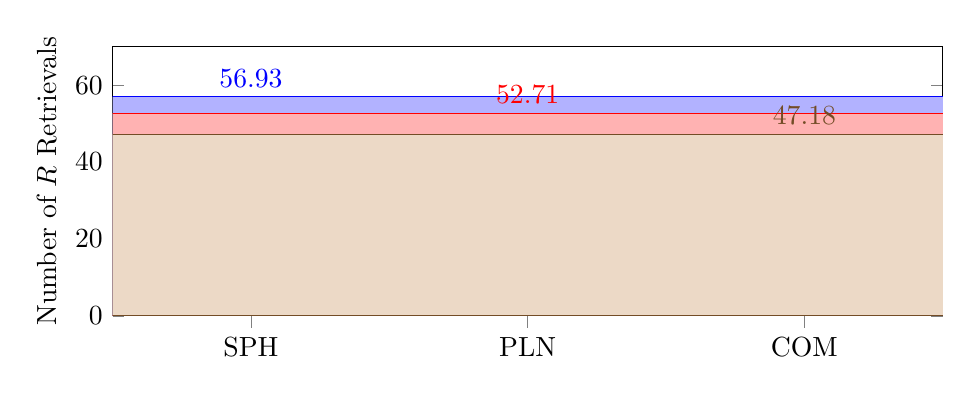
\begin{tikzpicture}
    \begin{axis}[
    ybar,
    width=\linewidth, height=5cm,
    ylabel={Number of $R$ Retrievals}, ylabel near ticks, ymin=0, ymax=70,
    xticklabels={SPH, PLN, COM},
    xtick={1, 2, 3}, xmin=0.5, xmax=3.5, xtick pos=left,
    nodes near coords, nodes near coords align={vertical},
    every axis plot/.append style={
    ybar,
    bar width=40,
    bar shift=0pt,
    fill
    }
    ]
        \addplot coordinates {(1, 56.93)}; % SPH
        \addplot coordinates {(2, 52.71)}; % PLN
        \addplot coordinates {(3, 47.18)};
    \end{axis}
\end{tikzpicture}

%SELECT AVG(QueryCount), IdentificationMethod
%FROM REDUCTION
%WHERE rowid IN (
%    SELECT rowid
%    FROM REDUCTION
%    WHERE (IdentificationMethod LIKE 'Plane' OR IdentificationMethod LIKE 'Sphere')
%    AND ShiftDeviation < 1.0e-3 AND ShiftDeviation > 1.0e-5 AND FalseStars = 0
%    AND QueryCount > 1
%)
%GROUP BY IdentificationMethod

%SELECT AVG(QueryCount)
%FROM REDUCTION
%WHERE rowid IN (
%    SELECT rowid
%    FROM REDUCTION
%    WHERE IdentificationMethod LIKE 'Composite'
%    AND ShiftDeviation < 1.0e-3 AND ShiftDeviation > 1.0e-5 AND FalseStars = 0
%    AND QueryCount > 1
%)
    \caption{
    Depicts the average number of catalog accesses required to obtain a $r$ set for methods with triangular
    features given $\rho = \ang{0.0001}$ of Gaussian noise.
    To characterize the pivoting method itself, we only display instances where $\abs{R} \neq 1$ with the first $b$
    selection.
    The Spherical Triangle method (SPH) has 1952 / 2000 runs matching the criteria before, the Planar Triangle
    method (PLN) has 1946 runs, and the Composite Pyramid (COM) method has 1957 runs.
    }\label{fig:rPivot}
    }
\end{figure}

\subsubsection{How expensive is the pivoting process?}
%import numpy as np
%m_1, m_2, s_1, s_2, n_1, n_2 = 52.71, 47.18, 56.794658219949106, 47.01765577951369, 1946, 1957
%z = (m_2 - m_1) / np.sqrt( ((s_1 * s_1) / n_1) + ((s_2 * s_2) / n_2) )
As seen previously, identification methods with triangular features have the most number of instances where
$\abs{R} = 1$ given an image with no noise.
In~\autoref{fig:rPivot}, the average number of catalog accesses are displayed for these same methods where the first
$b$ selection does not meet the $R$ criterion given an image with Gaussian noise.
We note that the average number of catalog accesses is higher in methods that use the pivoting processes,
as opposed to those that do not.
Given the null hypothesis that the difference between the Planar Triangle method's number of catalog accesses and
the Composite Pyramid method's number of catalog accesses is not significant, $z = 3.3, p < 0.0001$ is
obtained with a two-tailed two sample $Z$ test.
With the data collected here, we find that the pivoting process results in more catalog accesses on average.
This increased number of catalog accesses results in a $6.70\si{ms}$ difference on average between the two.

The pivoting process was only tested with methods using triangular features, whose candidate sets met the $R$ criterion
the most frequently.
An area of interest would be to see the effects of applying this process to methods with angular features (i.e.\ Angle,
Dot Angle, Pyramid).
These methods met the criterion less frequently, and would likely benefit from attempting to reduce the $R$ set before
deciding to choose another $b$ set.

\subsection{3rd Filter: Bijection}\label{subsec:3rdFilter:Bijection}
\begin{figure}
    \centering{
        \begin{tikzpicture}
    \begin{axis}[
    ybar,
    width=\linewidth, height=5cm,
    ylabel={Accuracy of $(f, b, r)$}, ylabel near ticks, ymin=0, ymax=1.3,
    xtick={1, 2, 3}, xticklabels={$\ang{0}$, $\ang{0.000001}$, $\ang{0.001}$},
    xlabel={$\sigma$ of Noise (degrees)}, xmin=0.5, xmax=3.5, xtick pos=left,
    nodes near coords, every node near coord/.append style={rotate=90, anchor=west},
    legend style={at={(0.5,-0.35)}, anchor=north,legend columns=-1},
    bar width=7
    ]
        \addplot coordinates {(1, 0.999416666666667) (2, 0.999222222222222) (3, 0.354333333333333)};
        \addplot coordinates {(1, 0.956083333333329) (2, 0.954444444444449) (3, 0.203166666666665)};
        \addplot coordinates {(1, 1.0) (2, 1.0) (3, 0.0)};
        \addplot coordinates {(1, 1.0) (2, 0.999833333333333) (3, 0.346333333333333)};
        \legend{PYR, PYR-N, COM, COM-N}
    \end{axis}
\end{tikzpicture}
        \caption{
        Depicts the frequency of correct bijections ($a(h, b, r)$) formed with and without the verification step of
        both the Pyramid and Composite Pyramid methods.
        There exists 2000 runs for each identification method, with a 500 catalog access limit.
        PYR corresponds to the Pyramid method with the verification step, PYR-N corresponds to the Pyramid method
        without the verification step, COM corresponds to the Composite Pyramid method with the verification step,
        and COM-N corresponds to the Composite Pyramid method without the verification step.
        }\label{fig:verify}
    }
\end{figure}

\begin{figure*} % HAD TO MOVE THIS GUY TOO...
    \centering{
    \begin{subfigure}[b]{0.48\linewidth}
        \begin{tikzpicture}
    \begin{axis}[
    ybar,
    width=\linewidth, height=5cm,
    ylabel={$t \ (\si{ms})$}, ylabel near ticks, ymin=10, ymax=100000,
    xtick={1, 2, 3}, xticklabels={$\ang{0}$, $\ang{0.0001}$, $\ang{0.01}$},
    xlabel={$\sigma$ (degrees)}, xmin=0.5, xmax=3.5, xtick pos=left, point meta=rawy,
    nodes near coords, every node near coord/.append style={rotate=90, anchor=west,
    /pgf/number format/.cd,fixed,precision=6},
    legend style={at={(0.5,-0.35)}, anchor=north,legend columns=-1},
    bar width=7, ymode=log, log origin=infty, max space between ticks=20
    ]
        \addplot coordinates {(1, 1197.43) (2, 1349.07) (3, 6509.00)};
        \addplot coordinates {(1, 160.68) (2, 161.80) (3, 872.22)};
        \addplot coordinates {(1, 323.94) (2, 339.23) (3, 392.29)};
        \addplot coordinates {(1, 324.35) (2, 328.85) (3, 352.24)};
        \addplot coordinates {(1, 170.79) (2, 171.53) (3, 364.04)};
        \addplot coordinates {(1, 405.53) (2, 1545.45) (3, 362.30)};
        \legend{ANG, INT, SPH, PLN, PYR, COM}
    \end{axis}
\end{tikzpicture}
    \end{subfigure}
    \begin{subfigure}[b]{0.48\linewidth}
        %if __name__ == '__main__':
%    from numpy import std, average, sqrt, polyfit, log
%    from sqlite3 import connect
%    from os import environ
%
%    conn_1 = connect(environ['HOKU_PROJECT_PATH'] + '/data/lumberjack-all-triad.db')
%    cur = conn_1.cursor()
%
%    # 1,   2,      3,      4,      5,     6,    7,   8
%    # 0.0, 1.0e-6, 1.0e-5, 0.0001, 0.001, 0.01, 0.1, 1.0
%
%    for d in [[1, 2, 3, 4, 5, 6, 7, 8], [0.0, 1.0e-6, 1.0e-5, 0.0001, 0.001, 0.01, 0.1, 1.0]]:
%        t = polyfit(log(d[3:]), [0.9725, 0.386, 0.0035, 0.0, 0.0], 1)
%        print('Angle: {}*ln(x) + {}'.format(t[0], t[1]))
%
%        t = polyfit(log(d[4:]), [0.9885, 0.7055, 0.033, 0.00383333333333333], 1)
%        print('Dot: {}*ln(x) + {}'.format(t[0], t[1]))
%
%        t = polyfit(log(d[2:]), [0.9715, 0.8135, 0.259, 0.0253333333333333, 0.0095, 0.00716666666666667], 1)
%        print('Sphere: {}*ln(x) + {}'.format(t[0], t[1]))
%
%        t = polyfit(log(d[2:]), [0.9865, 0.8615, 0.332166666666667, 0.0245, 0.0095, 0.00483333333333333], 1)
%        print('Plane: {}*ln(x) + {}'.format(t[0], t[1]))
%
%        t = polyfit(log(d[3:]), [0.999333333333334, 0.354333333333333, 0.0, 0.0, 0.0], 1)
%        print('Pyramid: {}*ln(x) + {}'.format(t[0], t[1]))
%
%        t = polyfit(log(d[1:]), [1.0, 0.65, 0.0035, 0.0, 0.0, 0.0, 0.0], 1)
%        print('Composite: {}*ln(x) + {}'.format(t[0], t[1])), print()

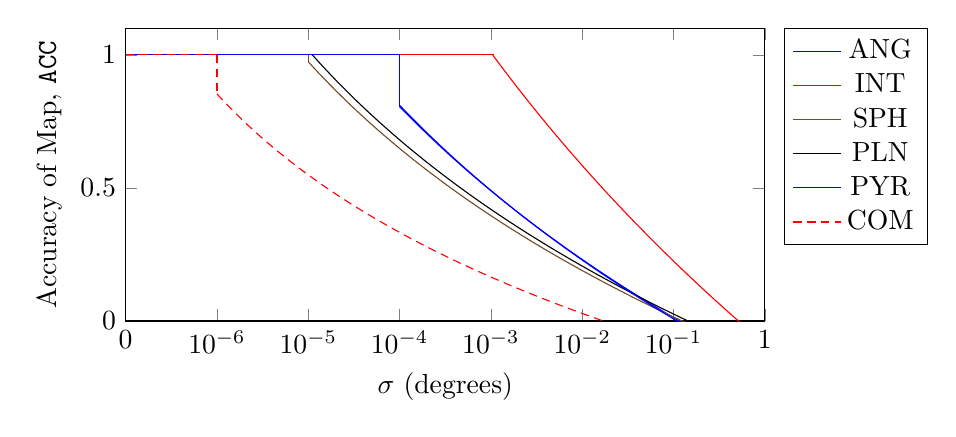
\begin{tikzpicture}
    \begin{axis}[
    width=0.8\linewidth, height=5.3cm,
    ylabel={Accuracy of Map, \texttt{ACC}}, ymin=0, ymax=1.1,
    xlabel={$\sigma$ (degrees)}, xmin=1, xmax=8,
    xtick={1, 2, 3, 4, 5, 6, 7, 8},
    xticklabels={$0$, $10^{-6}$, $10^{-5}$, $10^{-4}$, $10^{-3}$, $10^{-2}$, $10^{-1}$, $1$},
    samples=100, no markers, legend pos=outer north east, enlargelimits=false
    ]
        \addplot +[domain=1:4, forget plot]{1};
        \addplot +[forget plot] coordinates {(4, 1) (4, 0.8055384229041530)};
        \addplot +[domain=4:8]{-1.416887591459587*ln(x) + 2.7697617012853217};
        \addlegendentry{ANG}

        \addplot +[domain=1:5.03, forget plot]{1};
%        \addplot +[forget plot] coordinates {(5, 1) (5, 1)};
        \addplot +[domain=5.02:8]{-2.3292306442173216*ln(x) + 4.757244753386215};
        \addlegendentry{INT}

        \addplot +[domain=1:3, forget plot]{1};
        \addplot +[forget plot] coordinates {(3, 1) (3, 0.9738787471803161)};
        \addplot +[domain=3:8]{-1.1317828984553227*ln(x) + 2.217269347527745};
        \addlegendentry{SPH}

        \addplot +[domain=1:3, forget plot]{1};
%        \addplot +[forget plot] coordinates {(3, 1) (3, )};
        \addplot +[domain=3.04:8]{-1.1696544292494204*ln(x) + 2.301996347627258};
        \addlegendentry{PLN}

        \addplot +[domain=1:4, forget plot]{1};
        \addplot +[forget plot] coordinates {(4, 1) (4, 0.8105837347641904)};
        \addplot +[domain=4:8]{-1.4347255837709008*ln(x) + 2.7995357213002334};
        \addlegendentry{PYR}

        \addplot +[domain=1:2, forget plot]{1};
        \addplot +[forget plot] coordinates {(2, 1) (2, 0.8533960244900531)};
        \addplot +[domain=2:8]{-0.7510156659772902*ln(x) + 1.3739604159185614};
        \addlegendentry{COM}
    \end{axis}
\end{tikzpicture}
    \end{subfigure}
    \caption{
    Both plots represent some statistic about the resulting bijection $h$ produced by each identification method
    given some image with varying Gaussian noise.
    There exist 2000 runs for each identification method, with a 500 catalog access limit.
    The left plot depicts the average time to obtain $h$, and the right plot depicts the trend line
    $a(h, b, r) = A \cdot \mathit{ln}\left( \rho \right) + B$.
    }\label{fig:gaussianNoise}
    }
\end{figure*}

\subsubsection{How effective are additional verification steps?}
%if __name__ == '__main__':
%from numpy import std, average, sqrt
%from sqlite3 import connect
%from os import environ
%
%conn_1 = connect(environ['HOKU_PROJECT_PATH'] + '/data/lumberjack-all-triad.db')
%conn_2 = connect(environ['HOKU_PROJECT_PATH'] + '/data/lumberjack-pyramid-noverify.db')
%
%name = 'Pyramid'
%
%sample_1 = list(map(lambda b: b.execute("""
%SELECT PercentageCorrect
%FROM IDENTIFICATION
%WHERE ShiftDeviation < 1.0e-7 AND FalseStars = 0
%AND IdentificationMethod LIKE '{}'
%""".format(name)).fetchall(), [conn_1, conn_2]))
%
%sample_2 = list(map(lambda b: b.execute("""
%SELECT PercentageCorrect
%FROM IDENTIFICATION
%WHERE ShiftDeviation < 1.0e-5 AND FalseStars = 0
%AND IdentificationMethod LIKE '{}'
%""".format(name)).fetchall(), [conn_1, conn_2]))
%
%sample_3 = list(map(lambda b: b.execute("""
%SELECT PercentageCorrect
%FROM IDENTIFICATION
%WHERE ShiftDeviation < 1.0e-2 AND ShiftDeviation > 1.0e-4 AND FalseStars = 0
%AND IdentificationMethod LIKE '{}'
%""".format(name)).fetchall(), [conn_1, conn_2]))
%
%flatten = lambda a: [b[0] for b in a]
%for i, sample in enumerate([sample_1, sample_2, sample_3]):
%n_1, n_2 = 2000, 2000
%m_1, m_2 = average(flatten(sample[0])), average(flatten(sample[1]))
%s_1, s_2 = std(flatten(sample[0])), std(flatten(sample[1]))
%print('Z Score of {}: {}'.format(i, (m_2 - m_1) / sqrt( ((s_1 * s_1) / n_1) + ((s_2 * s_2) / n_2) )))

%import numpy as np
%print(np.average( [6.97725 - 3.00525, 6.9615 - 3.005, 398.0655 -  ))
In~\autoref{fig:verify}, the accuracy of the bijection produced by the Pyramid and Composite Pyramid methods are
displayed with and without the verification step for varying levels of Gaussian noise.
Without noise, the Pyramid method without its verification step is 4.33\% less accurate than the Pyramid method with
verification on average.
This behavior is consistently seen for Gaussian noise of $\rho=\ang{0.000001}$ \& $\rho=\ang{0.001}$, and
can be attributed to the more frequent rejection of bijections whose $R$ sets have met the criterion but whose resulting
$h$ would have been incorrect.
In the $\rho=\ang{0.001}$ case, there exists a difference of 389.95 accesses between both variations of the Pyramid
and a 15\% bijection accuracy difference in favor of the method with the verification step.
Given the null hypotheses that the difference between both variations of the Pyramid method are different for each level
of noise, $z_0 = 15.87, z_{0.000001} = 16.04, z_{0.001} = 12.14$ (all $p < 0.0001$) is obtained with two-tailed two
sample $Z$ tests.
The verification step increases the accuracy of the Pyramid method.

The response to Gaussian noise for the Composite Pyramid begins at $\rho=\ang{0.001}$, with a 34.6\% difference
between the two variants in favor of the method without the verification step.
Unlike the verification step in the Pyramid method, this filter appears to be too aggressive for the Composite Pyramid
method.
The variant without the verification step has an average of 193.93 catalog accesses at $\rho=\ang{0.001}$.
The Pyramid variant without the verification step only had an average of 8.114 catalog accesses, suggesting that the
$\abs{R} = 1$ criterion and the \Call{DMT}{} process are sufficient enough for rejecting incorrect $r$ sets and
bijections for the Composite Pyramid method.

\subsection{End to End}\label{subsec:endToEndEvaluation}
\subsubsection{Which method is the fastest given no noise?}
In~\autoref{fig:gaussianNoise}, the left plot depicts the end to end running time of each identification method given
varying degrees of Gaussian noise.
In the no noise case, the Angle method is the slowest identification method on average.
The next slowest method is the Composite Pyramid method, a factor of 2.95 times faster than the Angle method.
Recall that the Angle method had the fastest query step, but the largest $\abs{R}$.
On average, it takes 69.85 catalog accesses to obtain a bijection and 68.10 catalog accesses to obtain $r$.
This suggests that the Angle method's long running time stems from the $\abs{R} = 1$ criterion and not the \Call{DMT}{}
process.

%import numpy as np
%m_1, m_2, s_1, s_2, n_1, n_2 = 160.675, 170.7905, 0.53808, 0.52922, 2000, 2000
%z = (m_2 - m_1) / np.sqrt( ((s_1 * s_1) / n_1) + ((s_2 * s_2) / n_2) )
The fastest method in the noise case appears to be the Dot Angle method, with the second fastest method running
10.11\si{ms} slower.
There exists 0 / 2000 runs where the Dot Angle method runs above the Pyramid method's average running time
($170.79\si{ms}$) and the Dot Angle method has the fastest recorded identification run of 135ms.
The Dot Angle method is the fastest identification method given no noise.

\subsubsection{Which method is the fastest given varying levels of Gaussian noise?}
As Gaussian noise is increased from $\rho=\ang{0}$ to $\rho=\ang{0.01}$, the Angle method experiences the largest
response of $5311.57$ additional $\si{ms}$.
The next slowest method in the noise of $\rho=\ang{0.01}$ case is the Dot Angle method, a factor of 7.46 times faster
than the Angle method.
On average, the Angle method takes 399.66 catalog accesses to obtain a bijection and only 36.72 catalog accesses
to obtain $r$ here.
In the no noise case, this method's long running time can attributed to the aggressive $R$ criterion.
Given Gaussian noise, the \Call{DMT}{} process plays a larger role with the Angle method and returns to $b$
decision process more often.

The Composite Pyramid method shows an interesting runtime response to this type of noise, running $1139.92\si{ms}$
longer given $\ang{0.0001}$ of noise from no noise but $1183.15\si{ms}$ shorter from $\ang{0.0001}$ of noise to
$\ang{0.01}$.
The Pyramid method is observed to have this same running time response against noise at $\rho=\ang{0.001}$
(not depicted).
The most probable explanation lies in how far each run travels from the $b$ decision step.
At $\rho=\ang{0.0001}$, the Composite Pyramid has gone through the $\abs{R} = 1$ criterion and is likely choosing
another $b$ set after the verification step.
At $\rho=\ang{0.01}$, the Composite Pyramid is not passing the same criterion and does not waste as many catalog
accesses because the verification step is not being performed.

%if __name__ == '__main__':
%from numpy import std, average, sqrt
%from sqlite3 import connect
%from os import environ
%
%conn_1 = connect(environ['HOKU_PROJECT_PATH'] + '/data/lumberjack-all-triad.db')
%conn_2 = connect(environ['HOKU_PROJECT_PATH'] + '/data/lumberjack-pyramid-noverify.db')
%
%sample_1 = conn_1.execute("""
%SELECT TimeToResult
%FROM IDENTIFICATION
%WHERE ShiftDeviation > 1.0e-7 AND FalseStars = 0
%AND IdentificationMethod LIKE 'Plane'
%""").fetchall()
%
%sample_2 = conn_1.execute("""
%SELECT TimeToResult
%FROM IDENTIFICATION
%WHERE ShiftDeviation > 1.0e-7 AND FalseStars = 0
%AND IdentificationMethod LIKE 'Pyramid'
%""").fetchall()
%
%flatten = lambda a: [b[0] for b in a]
%n_1, n_2 = 12000, 12000
%m_1, m_2 = average(flatten(sample_1)), average(flatten(sample_2))
%s_1, s_2 = std(flatten(sample_1)), std(flatten(sample_2))
%print('Z Score of: {}'.format((m_2 - m_1) / sqrt( ((s_1 * s_1) / n_1) + ((s_2 * s_2) / n_2) )))
The fastest method on average given images with the set of Gaussian noise below is the Pyramid method at
$288.44\si{ms}$ (of 12000 runs).
\begin{equation}\label{eq:sigmasTested}
    \rho \in \set{10^{-1}, 10^{-2}, \ldots, 10^{-6}}
\end{equation}
The second fastest method given the same noise set is the Planar Triangle method at $341.16\si{ms}$.
Given the null hypothesis that the difference between both averages is not significant, $z = 24.32, p < 0.0001$ is
found with a two sample $Z$ test.
With the data collected here, the Pyramid method is the fastest method given varying amounts of Gaussian noise.

\begin{figure*} % NOTE: HAD TO MOVE THIS AWAY FROM THE FALSE STAR SECTION.
    \centering{
    \begin{subfigure}[b]{0.48\linewidth}
        \begin{tikzpicture}
    \begin{axis}[
    ybar,
    width=\linewidth, height=5cm,
    ylabel={$t \ (\si{ms})$}, ylabel near ticks, ymin=10, ymax=100000,
    xtick={1, 2, 3}, xticklabels={0, 6, 12},
    xlabel={$\omega$}, xmin=0.5, xmax=3.5, xtick pos=left, point meta=rawy,
    nodes near coords, every node near coord/.append style={rotate=90, anchor=west,
    /pgf/number format/.cd,fixed,precision=2},
    legend style={at={(0.5,-0.35)}, anchor=north,legend columns=-1},
    bar width=7, ymode=log, log origin=infty, max space between ticks=20
    ]
        \addplot coordinates {(1, 1197.43) (2, 1737.94) (3, 2431.58)};
        \addplot coordinates {(1, 160.68) (2, 209.36) (3, 280.54)};
        \addplot coordinates {(1, 323.94) (2, 355.54) (3, 386.20)};
        \addplot coordinates {(1, 324.35) (2, 350.60) (3, 390.41)};
        \addplot coordinates {(1, 170.79) (2, 183.71) (3, 195.53)};
        \addplot coordinates {(1, 405.53) (2, 685.07) (3, 972.04)};
        \legend{ANG, DOT, SPH, PLN, PYR, COM}
    \end{axis}
\end{tikzpicture}
    \end{subfigure}
    \begin{subfigure}[b]{0.48\linewidth}
        \begin{tikzpicture}
    \begin{axis}[
    ybar,
    width=\linewidth, height=5cm,
    ylabel={$a(f, b, r)$}, ylabel near ticks, ymin=0, ymax=1.4,
    xtick={1, 2, 3}, xticklabels={0, 6, 12},
    xlabel={$\omega$}, xmin=0.5, xmax=3.5, xtick pos=left,
    nodes near coords, every node near coord/.append style={rotate=90, anchor=west,
    /pgf/number format/.cd,fixed,precision=4},
    legend style={at={(0.5,-0.35)}, anchor=north,legend columns=-1},
    bar width=7
    ]
        \addplot coordinates {(1, 0.977) (2, 0.979) (3, 0.960)};
        \addplot coordinates {(1, 1.0) (2, 0.982) (3, 0.965)};
        \addplot coordinates {(1, 1.0) (2, 0.840) (3, 0.696)};
        \addplot coordinates {(1, 1.0) (2, 0.845) (3, 0.703)};
        \addplot coordinates {(1, 0.999) (2, 0.999) (3, 0.995)};
        \addplot coordinates {(1, 1.0) (2, 0.994) (3, 0.973)};
        \legend{ANG, DOT, SPH, PLN, PYR, COM}
    \end{axis}
\end{tikzpicture}
    \end{subfigure}
    \caption{
    Both plots represent some statistic about the resulting bijection $h$ produced by each identification method
    given some image with varying amounts of spikes $\omega$.
    There exist 2000 runs for each identification method, with a 500 catalog access limit.
    The left plot depicts the average time to obtain $h$, and the right plot depicts the average accuracy of $h$.
    }\label{fig:falseNoise}
    }
\end{figure*}

\subsubsection{Which method has the slowest growing $h$ accuracy response to increasing noise?}
The selection of the query $\sigma$ parameters play a significant role in accuracy of each method given images with
Gaussian noise.
For methods that query the catalog using on the $\theta$ feature (Angle, Dot Angle, Pyramid), the $\sigma$ parameter
serves as a rough upper bound for the amount of Gaussian noise tolerated.
%In~\autoref{fig:gaussianNoise}, the plot on the right depicts the accuracy of resulting bijection of each method for
%varying levels of Gaussian noise.
When the level of noise is equal to the Angle and Pyramid $\sigma_\theta$ parameter ($\ang{0.0001}$),
both methods have an average $h$ accuracy of $98.59 \pm 1.34\%$.
When Gaussian noise is increased to $\ang{0.001}$, both methods drop to $47.02 \pm 1.58\%$.

For methods with features that are not angular (Spherical Triangle, Planar Triangle, Composite Pyramid),
characterizing the effect of Gaussian noise becomes more difficult.
These methods have the query parameters $\sigma_a = 10^{-9}$ and $\sigma_\imath = 10^{-9}$, and first show an
accuracy response to noise at $\ang{0.00001}$.
%The Dot Angle method has the largest query $\sigma$ parameters, and only experiences a response to noise at
%$\ang{0.01}$.
%Given the current set of query $\sigma$, the Dot Angle is the most accurate method on average.

Ranking each method based their $h$ accuracy here is not too insightful, so instead we analyze the rate of change
involved with varying levels of noise.
The right plot in~\autoref{fig:gaussianNoise} depicts the trend line for all methods where $h$ accuracy is displayed
against the amount of Gaussian noise.
Each line was fit to the equation below using least squares:
\begin{equation}
    a(f, b, r) =
    \begin{cases}
        0 & \rho < 0 \\
        1 & 0 \leq \rho < \rho_c \\
        A \cdot \mathit{ln}(\rho) + B & \rho \geq \rho_c
    \end{cases}
\end{equation}
where $A$ and $B$ are the parameters found with the regression, $a(f, b, r)$ is the accuracy of the bijection, and
$\rho_c$ is the point where $a(f, b, r)$ is observed to dip below 95\%.
The acceleration of the accuracy varies across methods through the value of $A$:
\begin{equation}
    \frac{d^{2}a(f, b, r)}{d\rho^2} = \frac{-A}{\rho^2}
\end{equation}
A larger $A$ suggests that a change in query $\sigma$ or Gaussian noise will not affect the accuracy of the method
as much as a method with a larger $A$.
The method with the largest acceleration toward $0\%$ $h$ accuracy is the Dot Angle method ($A = -0.15749$) .
The Spherical Triangle method has the slowest growing $h$ accuracy response to increasing noise ($A = -0.09266$).

\subsubsection{Which method is the fastest given varying \\ amounts of false stars?}
In~\autoref{fig:falseNoise}, the plot on the left depicts the end to end running time of each method given varying
amounts of spikes.
As the number of spikes increases from 0 to 12, the Angle method again experiences the largest response of
$1234.15\si{ms}$.
The next slowest method is the Composite Pyramid method, a factor of 2.50 times faster than the Angle method.
The difference between the 1st and 2nd slowest methods is 2.98 times less than the Gaussian noise case.
On average, it takes 114.23 catalog accesses to obtain $h$ and only 54.85 accesses to obtain $r$.
Relative to the Gaussian noise comparison, \Call{DMT}{} and $\abs{R} = 1$ criterion play a more equal role in
the decision to choose a new $b$ set.

%if __name__ == '__main__':
%from numpy import std, average, sqrt
%from sqlite3 import connect
%from os import environ
%
%conn_1 = connect(environ['HOKU_PROJECT_PATH'] + '/data/lumberjack-all-triad.db')
%conn_2 = connect(environ['HOKU_PROJECT_PATH'] + '/data/lumberjack-pyramid-noverify.db')
%
%sample_1 = conn_1.execute("""
%SELECT TimeToResult
%FROM IDENTIFICATION
%WHERE FalseStars > 0
%AND IdentificationMethod LIKE 'Pyramid'
%""").fetchall()
%
%sample_2 = conn_1.execute("""
%SELECT TimeToResult
%FROM IDENTIFICATION
%WHERE FalseStars > 0
%AND IdentificationMethod LIKE 'Dot'
%""").fetchall()
%
%flatten = lambda a: [b[0] for b in a]
%n_1, n_2 = 8000, 8000
%m_1, m_2 = average(flatten(sample_1)), average(flatten(sample_2))
%s_1, s_2 = std(flatten(sample_1)), std(flatten(sample_2))
%print('Z Score of: {}'.format((m_2 - m_1) / sqrt( ((s_1 * s_1) / n_1) + ((s_2 * s_2) / n_2) )))
The fastest method on average given images with the set of spikes below is the Pyramid method at $186.22\si{ms}$
(of 8000 runs).
\begin{equation}\label{eq:numberOfSpikes}
    \omega \in \set{ 3, 6, 9, 12 }
\end{equation}
The second fastest method given the same noise set is the Dot Angle method at $228.37\si{ms}$.
Given the null hypothesis that the difference between both averages is not significant, $z = 28.47, p < 0.0001$ is
found with a two sample $Z$ test.
The Pyramid method is the fastest method given varying amounts of spikes.
The process for choosing distinct image star sets is shown to be effective in finding a bijection that meets the Pyramid
criteria the fastest.

%if __name__ == '__main__':
%from numpy import std, average, sqrt, polyfit, log
%from sqlite3 import connect
%from os import environ
%
%conn_1 = connect(environ['HOKU_PROJECT_PATH'] + '/data/lumberjack-all-triad.db')
%cur = conn_1.cursor()
%
%for name in ['Angle', 'Dot', 'Sphere', 'Plane', 'Pyramid', 'Composite']:
%sample_1 = list(map(lambda a: a[0], cur.execute("""
%SELECT AVG(TimeToResult)
%FROM IDENTIFICATION
%WHERE FalseStars > 0
%AND IdentificationMethod LIKE ?
%GROUP BY FalseStars
%ORDER BY FalseStars
%""", (name, )).fetchall()))
%
%t = polyfit([3, 6, 9, 12], sample_1, 1)
%print('{name}: {t_0}*x + {t_1}'.format(name=name, t_0=round(t[0], 5), t_1=round(t[1], 5)))
Each method exhibits an increase to runtime as additional spikes are added.
To characterize how each method's runtime grows with increasing false stars, each method's runtime was fit to a linear
equation using least squares:
\begin{equation}
    t = A\cdot\omega + B
\end{equation}
where $A$ and $B$ are the parameters found with the regression and $t$ is the end to end running time of the method.
A smaller $\abs{A}$ suggests that the number of spikes will affect the end to end runtime than that of a method with a
larger $\abs{A}$.
The method with the largest $\abs{A}$ is the Angle method with $A = -414.559$.
The method with this smallest $\abs{A}$ term is the Pyramid method with $A = -6.766$.
The Pyramid method is the fastest given varying amounts of false stars, whose runtime is also the least responsive to
increasing spikes.

\subsubsection{Which method is the most accurate given varying amounts of false stars?}
%if __name__ == '__main__':
%from numpy import std, average, sqrt
%from sqlite3 import connect
%from os import environ
%
%conn_1 = connect(environ['HOKU_PROJECT_PATH'] + '/data/lumberjack-all-triad.db')
%conn_2 = connect(environ['HOKU_PROJECT_PATH'] + '/data/lumberjack-pyramid-noverify.db')
%
%sample_1 = conn_1.execute("""
%SELECT PercentageCorrect
%FROM IDENTIFICATION
%WHERE FalseStars = 12
%AND (IdentificationMethod LIKE 'Plane' OR IdentificationMethod LIKE 'Sphere')
%""").fetchall()
%
%sample_2 = conn_1.execute("""
%SELECT PercentageCorrect
%FROM REDUCTION
%WHERE FalseStars = 12
%AND (IdentificationMethod LIKE 'Plane' OR IdentificationMethod LIKE 'Sphere')
%""").fetchall()
%
%flatten = lambda a: [b[0] for b in a]
%n_1, n_2 = 2000, 2000
%m_1, m_2 = average(flatten(sample_1)), average(flatten(sample_2))
%s_1, s_2 = std(flatten(sample_1)), std(flatten(sample_2))
%print('Z Score of: {}'.format((m_2 - m_1) / sqrt( ((s_1 * s_1) / n_1) + ((s_2 * s_2) / n_2) )))
In~\autoref{fig:falseNoise}, the plot on the right depicts the average accuracy of each bijection given varying amounts
of spikes.
As the number of false stars is increased from $\omega = 0$ to $\omega = 12$, the methods that experience the largest
$h$ accuracy response are the Spherical Triangle method ($30.42\%$ average decrease) and the Planar Triangle method
($29.68\%$ average decrease).
The average accuracy of the $r$ selection is a few percent less than the average accuracy of $h$ here
($0.53 \pm 1.78\%$ for both methods).
Given the null hypothesis that the difference between the accuracy of the $h$ bijection and the accuracy of the $r$
selection is not significant, $z = 0.37, p = 0.71$ was found with a two-tailed two sample $Z$ test.
There does not exist enough data to reject this hypothesis with $\alpha = 0.01$.
This suggests that the \Call{DMT}{} process is neither helpful or detrimental to the end to end accuracy of these
methods.

Ruling out the \Call{DMT}{} process, the most likely source of error for the triangle methods is their decision of
different $b$ sets.
If a false star exists as $b_1$ in $b$, the triangle methods will have to iterate through $n^2$ combinations and $n - 3$
pivots at most to choose another star that is not the spike.
The Angle method only has to wait $n$ additional combinations at most if a false star exists in $b$.
The Dot Angle method is able to get around the spike persistence problem by choosing $b$ sets based on their $\theta$
proximity to the central star $b_c$.
The Pyramid and Composite Pyramid methods have their $b$ decision process designed for this situation, increasing the
average turnover of all stars in the $b$ set.

The Pyramid method has the most accurate $h$ on average given images with $\omega$ in~\autoref{eq:numberOfSpikes}
at $99.84 \pm 3.53\%$.
The second most accurate method is the Composite Pyramid method at $99.19 \pm 8.95\%$.
Given the null hypothesis that the difference between the $h$ accuracies of both methods is not significant,
$z = 3.02, p = 0.003$ with a two-tailed two sample $Z$ test.
At $\alpha = 0.01$, our hypothesis does not hold true.
The Pyramid method is the most accurate under varying amounts of spikes.

	\section{Conclusion}\label{sec:conclusion}
Attitude determination is a vital part of all spacecraft missions.
Previously, devices such as magnetometers and Sun sensors would give one observation each in both the body and inertial
frames.
The advantage of star trackers is the presentation of multiple observations with just one device.
Star identification is the process associated that maps observations found in the body frame (i.e.\ the image) to the
inertial frame (i.e.\ the catalog).

Gottlieb's Angle method, Liebe's Dot Angle method, Motari's Pyramid method, Cole and Crassidis's Spherical and
Planar Triangle method, and Toloei's Composite Pyramid method were adjusted to fit a general identification flow
and were analyzed in terms of their query, reduction, and identification steps.
Portions that were interchangeable amongst all methods such as database access and centroid determination were
normalized or removed to focus on the star identification aspect itself.

In all experiments, the Pyramid method ranked first (or close to first) in running time and fairly high in accuracy.
The average short running time is a result of a relatively fast query step, and its accuracy can be attributed to the
verification procedure at identification time.
The Pyramid method is the least sensitive to hyperparameter changes in terms of query size response and accuracy
response.
This method produced the lowest number of catalog candidate sets for a given query, and is the most tolerant of
both Gaussian noise and false stars.

The Angle method had the fastest query step, which stems from the small catalog ($\sim$35 times smaller than
the next larger catalogs, the triangle catalogs).
There were a few instances where the accuracy of the Angle method was greater than the Pyramid method, but this came
at the cost of runtime.
The results produced by the query step heavily impacted the reduction and identification runtime.
For the no noise end-to-end case, this method was a factor of MP200 times slower than the next slowest method (Dot
Angle method).

The Dot Angle method is the most sensitive to hyperparameter changes, but had a larger ideal region than the other
methods.
The catalog for this method was $\sim$105 times larger than the Angle method, and consequently had the longest query
step.
This method handles Gaussian noise the best of all other methods, being the second fastest to identify an image and
being first in how accurate the result is.
In terms of false stars, this method ranks last in accuracy.

The accuracy of the Spherical and Planar Triangle methods rank in between for both Gaussian noise and false stars.
The differences between the spherical and planar triangle features are minuscule compared to the algorithms
encapsulating the features themselves.
These methods produced the smallest amount of candidates on average, which was useful in mitigating the highest
theoretical upper bound for catalog accesses.
Unfortunately, these methods were not the fastest nor were they the most accurate.

The Composite Pyramid method, a composite of the Planar Triangle method's features and the Pyramid method's processes,
ranks last in accuracy and average runtime for images with Gaussian noise 2nd in accuracy for images with just
false stars.
Combining the two methods also means combining the filters associated with each, and the results show inconsistent
runtime due to failing at different stages of the algorithm.
Instead of getting the best of both worlds here, the Composite Pyramid method inherits the worst portions of the two.

Overall, the Pyramid method handles both Gaussian noise and false stars the best in a reasonable amount of time.
If one is working with a small field-of-view with limited stars to choose from and Gaussian noise, the Dot Angle
method works best for using one less star than the Pyramid method.
If speed is not a factor but the field-of-view problem still persists, the Angle method should suffice.
    %\section{Acknowledgements}\label{sec:acknowledgements}
\begin{acks}
	We would like to thank Dr. Miguel Nunes, Eric Pilger, and Yosef Ben Gershom from the Hawaii Space Flight Laboratory for providing input toward the creation of software for a first generation star tracker.
\end{acks}
    \balance

%	\nocite{*}
	\bibliographystyle{ACM-Reference-Format}
	\bibliography{include/references}

\end{document}
